\documentclass[autodetect-engine,dvipdfmx-if-dvi,ja=standard,a5paper,10.5pt,twoside,openany,layout=v2]{bxjsbook}

\newcommand{\stypath}{./sty}
\newcommand{\articlepath}{./articles}
\newcommand{\assetspath}{./assets}

\newcommand{\jumpakuasset}{\assetspath/jumpakuasset}
\newcommand{\takuzooasset}{\assetspath/takuzoo3868asset}
\newcommand{\lrfasset}{\assetspath/lrf141asset}
\newcommand{\materialofmouseasset}{\assetspath/mouse/gray}
\newcommand{\keisukeasset}{\assetspath/keisuke495500asset}
\newcommand{\chikuwaitasset}{\assetspath/chikuwa_ITasset/gray}
\newcommand{\arunekoasset}{\assetpath/aruneko}

\usepackage{\stypath/localst17}
\usepackage{\stypath/mymintedsetting}

\usepackage{lipsum}
\usepackage{layout}

%Takuzoo3868
\usepackage{dirtree}

%Jumpaku
\usepackage{pxrubrica}
\usepackage{pxjahyper}
\usepackage{comment}
\usepackage{verbatim}

%materialofmouse
\usepackage{siunitx}

\title{LOCAL STUDENTS ヤバい同人誌執筆合宿}
\author{うっひょい \and ちくうぇいと \and あわあわ \and けんつ \and さわだ \and Jumpaku \and あるねこ}

\date{\today}

\begin{document}
\frontmatter
\maketitle
\begin{myintroduce}{\keisukeasset/my_twitter_icon_gray.jpg}{うっひょい}
  \LaTeX 大好き人間です.この前は\LaTeX でニューラルネットワークとか
  実装しました.デレマスの赤城みりあちゃんのプロデューサーを務めると共に
  龍崎薫ちゃんの先生もやっています.\\
  ブログ:\url{http://muscle-keisuke.hatenablog.com/}
\end{myintroduce}
\begin{myintroduce}{\chikuwaitasset/icon.jpg}{ちくうぇいと}
  RubyでイケイケWEBエンジニアになるつもりだったのに, 気がついたらmrubyをOSの下に組み込んだりして完全にシステムプログラミング沼に落ちてしまいました。\\
  どうしてこうなった。
\end{myintroduce}
\begin{myintroduce}{\materialofmouseasset/icon.png}{あわあわ}
  昔はプログラミングとかしてました。\\
  今は何もしてません。\\
  欲しいものリスト:\url{http://amzn.asia/edWsM}
\end{myintroduce}
\begin{myintroduce}{\lrfasset/icon_gray.jpg}{けんつ}
  カーネルからWebまで色々やってます。\\
  インフラとScalaとJavaが大好物です。
\end{myintroduce}
\begin{myintroduce}{\takuzooasset/takuzoo_gray.png}{さわだ @takuzoo3868}
  北の国に生きるコタツ星人.\\
  セキュリティまわりが好き,興味が湧いたらとりあえず手を動かす.takuzooの由来は叔父に貸したポケモンにて,返ってきたときに付けられていた名前から.
\end{myintroduce}
\begin{myintroduce}{\jumpakuasset/JumpakuMark_250x250_gray.png}{Jumpaku}

\end{myintroduce}

\begin{myintroduce}{./assets/aruneko/icon_gray.jpg}{あるねこ}
  この本の言い出しっぺで、LOCAL学生部の前部長。いつもはTwitterに生息中。
  もし第2弾があればまた手に取ってくれるとありがたいです!
\end{myintroduce}

\chapter{はじめに}
LOCALがくせーぶの紹介とかなんか.部長!お願いしますよ! by さわだ


\tableofcontents
\mainmatter
\chapterauthor{うっひょい}
\chapter{\LaTeX の乱数生成アルゴリズムを \\ 改善する}
\section{乱数とは}
乱数とはランダムな数のことを言い,乱数の数列を乱数列と言います.
乱数列は生成した数から次に生成する数を予測することができないことや,
非周期的などの性質があります.
乱数は原始の崩壊による放射線の輻射レベルや時間間隔,
抵抗器の熱雑音などの物理現象の中で観測することが出来ます.
自然現象から観測できる乱数を真の乱数または自然乱数などと言います.

乱数は現在,数値計算や物理現象のシミュレーション,
暗号化などに使われており,計算機上で生成する需要が高まっています.
しかし,計算機は決定的オートマトンなため,数値の計算は
確率的にしか行えず,真の乱数を生成することができません.
よって,現在は統計的に真の乱数と近似の性質を持つ数列を
生成する方法があり,その方法を疑似乱数アルゴリズムと言い,
疑似乱数アルゴリズムによって生成された数を疑似乱数と言います.

現在,世に出回っている疑似乱数アルゴリズムは様々あります.
これは今まで研究されてきたアルゴリズムに何かしらの問題があるからです.
偏りが出たり,パターンがあったり様々です.
また,疑似乱数には周期があります.
一定の数の乱数を出力したらまた,
最初から同じ疑似乱数列を出力し始めます.
現在は計算機のスペックも高くなりより複雑なシミュレーションを
行えるようになりました.
その為,用いられる疑似乱数の数が従来のアルゴリズムでは
周期を上回る危険性もありました.
周期を伸ばすことも新しい疑似乱数アルゴリズムを開発する理由の一つです.

乱数の歴史は長く,現在では様々なプログラミング言語に
標準で実装されています.
しかし,標準で実装されている疑似乱数アルゴリズムも
言語によってまちまちです.昔からあるプログラミング言語の場合,
標準実装されているアルゴリズムも昔のものである場合が多く,
いわゆる問題点があるアルゴリズムであることもあります.
本章ではプログラミング言語の中でも\LaTeX に実装されている
疑似乱数アルゴリズムについて解説し,
改善するためにモダンな疑似乱数アルゴリズムを\LaTeX で実装していきます.
\section{乱数生成コマンド}
\LaTeX のパッケージに固定小数演算ができるFPパッケージがあります.
\subsection{固定小数演算}
\TeX ,\LaTeX は共に整数の演算は可能ですが,小数点を含む計算は行うことができません(寸法を除く).
固定小数点の演算をすることを目的としてあるのがFPパッケージです.
\subsection{乱数を出力するFPrandomコマンド}
fpパッケージの中には上記以外にも$0\sim 1$の範囲の疑似乱数を出力するFPrandomというコマンドがあります.
FPseedでシード値を決めてからFPrandomを使って変数に乱数を格納します.
\begin{texcode}
\FPseed = 156
\FPrandom{\result}
\FPprint{\result}
\end{texcode}

\section{FPrandomの乱数生成アルゴリズムを調べる}
\subsection{目的}
今回はFPrandomに使われている疑似乱数がいわゆる多くの問題点がある昔のアルゴリズムかどうかを調べる為に行います.

\subsection{ソースを読む}
それではfpパッケージのソースを読んでいきます.
しかし,実際にはfpパッケージ本体が内部的に呼び出しているfp-randomパッケージのソースを読んでいきます.

\subsubsection{コメントに正解が書いてあった}
22行目からFPrandomの定義が始まります.その直後,コメントが長く続いています.
コメントには次のようなことが書かれていました.
\begin{quote}
Algorithm reproduce from a very old Fortran program (unknown origin!)
\end{quote}
どうやら大昔のFortranの疑似乱数アルゴリズムを\TeX に起こしたものがFPrandomの正体みたいですね.
これはいろいろ問題点がありそうですね.
更にその下のコメントにはFortranで書かれた疑似乱数アルゴリズムらしきものがあります.
これを読んでいけばどんなアルゴリズムが使われているか分かりますがそれではつまらないので
コメントを抜けた後の\TeX で書かれた疑似乱数アルゴリズムの方を見ていきましょう.

\subsubsection{\TeX のマクロで実装された疑似乱数アルゴリズム}
\begin{texcode}
\ifnum\FPseed=0%
     \FPseed=123456789%
     \FP@debug{random: seed value undefined! We will used \the\FPseed.%
        Define it if you want to generate a different sequence of random numbers.}%
\else%
     \FP@debug{random: seed value used: \the\FPseed}%
\fi%
\end{texcode}
これはシードを指定してるかどうかを判定してしてない場合123456789をシードとするというマクロですね.
次見ていきます.
\begin{texcode}
\FP@xia=\FPseed%
\divide\FP@xia by 127773%
\FP@xib=\FP@xia%
\multiply\FP@xib by 127773%
\advance\FP@xib by -\FPseed%
\FP@xib=-\FP@xib%
\multiply\FP@xia by 2836%
\FPseed=\FP@xib%
\multiply\FPseed by 16807%
\advance\FPseed by -\FP@xia%
\end{texcode}
このアルゴリズムのコアとなる乱数の計算ですね.\TeX で書いてる為ごちゃごちゃしていますが
数式で表すと以下のようになります.

\[
S_{n+1} = - \frac{S_n}{127773}\times 2836 + (16807S_n \bmod 127773)
\]
$S_n$が$n$番目に出力した乱数で$S_{n+1}$は$n+1$番目に出力する乱数です.つまり漸化式になっています.
線形合同法の漸化式と似ていますね.
線形合同法はC言語のrand関数に採用されているアルゴリズムですが多くの問題点が発見されていて現在は非推奨となっています.
線形合同法では$16807S_n$の部分が定数ですが,それが乱数を含む形になっています.
線形合同法の式は以下のとおりです.

\[
S_{n+1}=(A\times S_n + B) \bmod M \quad \textrm{(A,B,Mは定数)}
\]

...構造が非常に似ていますね.

\begin{texcode}
 \ifnum\FPseed>0%
  \else%
      \advance\FPseed by 2147483647%
  \fi%
  \FPdiv\FP@tmpa{\the\FPseed}{2147483647}%
  \global\let\FP@tmp\FP@tmpa%
  \global\FPseed=\FPseed%
\end{texcode}
乱数の正規化を行っています.$2147483647(=2^{32}-1)$がこの乱数列における最大値$M$で
この時点で$n+1$番目の乱数が負の値の場合は$M$を乱数に足します.
その後FPdivと呼ばれる小数の割り算ができるマクロによって乱数を$M$で割り,乱数を$0\sim 1$の範囲の値に正規化しています.
\begin{texcode}
  \let#1\FP@tmp%
\end{texcode}
最後に,FPrandomの第一引数に算出した乱数を代入して終了です.
\subsubsection{実際に出力してみる}
前節でFPrandomは線形合同法が用いられていることが分かりました.
しかし,線形合同法は実装が簡単にできる分,構造が単純で,
偏りが出たり,周期が短いことが問題となっています.
この節では,その問題点がFPrandomコマンドにも起こり得ることを検証していきます.
まずは周期性ですが,線形合同法の周期は$M-1$です.
FPrandomは$M=214793647$なので周期は$214793646$となります.
つまり,FPranndomコマンドを$M$回呼び出すと最初の乱数と一致することになります.


\chapterauthor{chikuwait(ちくうぇいと)}
\chapter{超入門 仮想化技術}
\section{はじめに}
近年, コンテナ型仮想化の普及もあり仮想化技術という存在を様々な場面でよく聞くようになりました. しかし, コンテナ型仮想化技術以外の他の仮想化技術というのは中々個人で扱うような技術・ソフトウェアではないこともあり, あまり知られていないことが多かったりします. また, コンテナ型仮想化技術も便利で環境構築が魔法のようなすごい存在といった漠然とした解釈の人もきっと多いはずです. そこでこの章では, 各種仮想化技術の仕組みや特徴について触れながらふわっと仮想化技術について紹介します.

\section{仮想化技術とは}
仮想化技術にはいくつか種類がありますが, この章では計算機資源を抽象化してOSなどに見せるプラットフォーム仮想化のことを指します. 仮想化することで複数の計算機資源を単一に見せたり, 単一の計算機資源を複数に見せることができます. そしてプラットフォーム仮想化を支えるための技術としてシステム仮想機械(VM, Virtual Machine)と呼ばれる計算機資源をエミュレートするソフトウェアが存在します. 仮想機械の実装は仮想マシンモニタ(VMM, Virtual Machine Monitor)を始めとしていくつか存在します. 例えば仮想専用サーバ(VPS, Virtual Private Server)のようなサービスでは図2.1にように, 物理サーバ上に仮想化OSによって複数の仮想サーバに分割してユーザに各仮想サーバを提供しています.
\begin{figure}[htbp]
    \centering
    \includegraphics[width=50mm]{./assets/chikuwa_ITasset/vps.png}
    \caption{hogehoge}
    \label{fig:one}
\end{figure}

\section{VMMについて}
仮想化を実現するVMMにはハイパーバイザ型(Type1),ホスト型(Type2)の2つに分類されます.

\subsection{ハイパーバイザー型(Type1)}
ハイパーバイザ型(Type1)は, ハードウェアの上で直接動作します. この方式ではホストOSと呼ばれるような土台になるOSが存在しないため,仮想マシンによる遅延や速度低下を防ぐことができます. そしてベアメタルハイパーバイザでは実装手法でもモノリシックカーネル型とマイクロカーネル型の2つに分類することができるほか, 仮想化のアプローチで完全仮想化と準仮想化に分類することができます.
\subsubsection{モノリシックカーネル型}
主にVMware ESX/ESXiなどで採用されている方式で, モノリシックという英語で「1枚岩」という意味の通り、VMMの中にデバイスドライバが含まれています. VMMがストレージをはじめ,ネットワークや入力デバイスといったハードウェアへのアクセスをすべてを処理します. この方法の利点はVMMとデバイスドライバが密接に連携するため,オーバーヘッドが少なく効率的です. しかしながら, VMMの中にデバイスドライバが存在しているため,ハイパーバイザ層でデバイスドライバを用意する必要があります. そのため, ハードウェアのサポートがマイクロカーネル型と比較して少なく, 使用するハードウェアに制限がかかってしまう場合があります. また, デバイスドライバをVMMに直接組み込むため, バグや脆弱性はVMM全体に広がってしまいます.
\begin{figure}[htbp]
    \centering
    \includegraphics[width=50mm]{./assets/chikuwa_ITasset/monolithic.png}
    \caption{モノリシックカーネル型ベアメタルハイパーバイザ}
    \label{fig:one}
\end{figure}
\begin{figure}[htbp]
    \centering
    \includegraphics[width=50mm]{./assets/chikuwa_ITasset/monolithic.png}
    \caption{モノリシックカーネル型のハードウェアアクセス}
    \label{fig:two}
\end{figure}
\subsubsection{マイクロカーネル型}
主にXenやHyper-Vで採用されている方式で, ハイパーバイザを管理する仮想マシンと管理OSを用意します. この管理OSはLinuxはWindows Serverなど汎用OSを使用します. また, 管理OSはXenではドメイン0, Hyper-Vでは親パーティションと呼ばれています. この方式では, デバイスドライバはVMMではなく, VMM上の仮想マシンとして動作している管理OSのデバイスドライバを使用します. 仮想マシンからハードウェアにアクセスする時はゲストOSから仮想デバイスのインターフェースを経由してVMMから管理OSに渡されます. そして管理OSのデバイスドライバからハードウェアにアクセスします.この方法は, 汎用OSのデバイスドライバを使用することで, モノリシックカーネル型に比べてハードウェアのサポートが多く, ハードウェアの対応が柔軟であるという利点があります. 例えば, Hyper-VならWindows用のデバイスドライバを使用することができます. しかしながら, ハードウェアにアクセスする際にVMMから管理OSを経由するため, モノリシックカーネル型よりも性能が低下してしまいがちであり, 管理用の汎用OSがクラッシュした場合全てのVMがクラッシュしてしまうといった欠点が存在します.
\begin{figure}[htbp]
    \centering
    \includegraphics[width=50mm]{./assets/chikuwa_ITasset/monolithic.png}
    \caption{マイクロカーネル型ベアメタルハイパーバイザ}
    \label{fig:one}
\end{figure}
\begin{figure}[htbp]
    \centering
    \includegraphics[width=50mm]{./assets/chikuwa_ITasset/monolithic.png}
    \caption{マイクロカーネル型のハードウェアアクセス}
    \label{fig:two}
\end{figure}

\subsubsection{完全仮想化}
完全仮想化方式のVMMでは, ハードウェアの挙動をすべてエミュレートします. そのため, 何も変更も加えていないそのままのホストOSを動かすことができます. 1960年代にIBMが「トラップアンドエミュレート」とよばれる方法で完全仮想化を実装しようとしました. この方法ではゲストOSが特権がない状態(Ring3)で実行させ, 特権(Ring0)が必要な命令を実行しようとすると失敗します. その際にVMMがその失敗をトラップして原因を確認してからその命令をエミュレートすることによってゲストOSの期待する結果を返すことができ, ゲストOSにRing0以外で実行されていることを気づかせないようにすることができます. しかしながら, この手法は古典的ですべてのアーキテクチャに適用できるわけではありませんでした. 特にx86プロセッサの場合, ユーザ権限で実行できるセンシティブ命令と呼ばれる計算機資源の構成などの依存している命令が存在しているため, 実装を難しくさせていました. そこで, 「バイナリトランスレーション」と呼ばれる新しい手法が使われるようになりました. この手法では, センシティブな命令以外の命令は直接CPUで実行し, センシティブな命令はVMMで実行前に動的に他の命令に置き換えられます.
\begin{figure}[htbp]
    \centering
    \includegraphics[width=50mm]{./assets/chikuwa_ITasset/monolithic.png}
    \caption{バイナリトランスレーション}
    \label{fig:one}
\end{figure}
\subsubsection{準仮想化}
\subsection{ホスト型(Type2)}


\chapterauthor{あわあわ}
\chapter{ほげ}
\section{自己紹介}
こんにちは、あわあわくん()(@materialofmouse)です。
同人誌を書く話になったのでLEDでひたすら発電してみました。
この章ではLEDで発電という普通はやらないことをやっています。
それに検証性がないのでちゃんと書かれてません。おまけだとおもって読んでください。

\section{LEDで発電できるの?}
できます。
詳しい話はインターネットで出てきますので、興味があるかたはぜひ調べてみてください。


\section{実際に発電してみる}
LEDで発電できるのか、実際に試したいと思います。
ものが近くにある方はぜひやってみてください。
\begin{description}
  \item[場所]{近くの駐車場}
  \item[時間]{14:10}
  \item[光源]{太陽光}
  \item[照度]{$160,000\si\lux$}
  \item[天気]{雲ひとつない晴れ}
\end{description}


\subsection{LED1個}
まず、LEDを1個。アノード側にテスターのプラス、カソード側にテスターのマイナスを接続します。
図\ref{fig:led1}の状態でLEDを太陽の方へ向けてみます。そこで発生した電流と電圧の値を取っていきます。
手元の環境では、普通の白色LEDから約10$\mu\si\ampere$,約1.2$\si\volt$発生しました。

\begin{figure}[htbp]
    \centering
    \includegraphics[width=60mm]{./assets/mouse/gray/a.JPG}
    \caption{LED1個で電流と電圧を測定している様子}
    \label{fig:led1}
\end{figure}

\subsection{直列と並列どちらが良いのか考える}
先ほどはLED1個で発電してみましたが、次は複数接続してみたいと思います。
複数接続にあたり、直列接続と並列接続のどちらが発電に適しているのかを実験してみました。

LED2個を直列に接続し、その両端をテスターで見ていきます。
図\ref{fig:led2}に測定の様子を示します.
そこに光を与えたところ、約100$\mu\si\ampere$,約2.5$\si\volt$発生しました。
この結果から、LED1個の時と比べ、電流、電圧ともに2倍になっていることがわかります。

\begin{figure}[htbp]
    \centering
    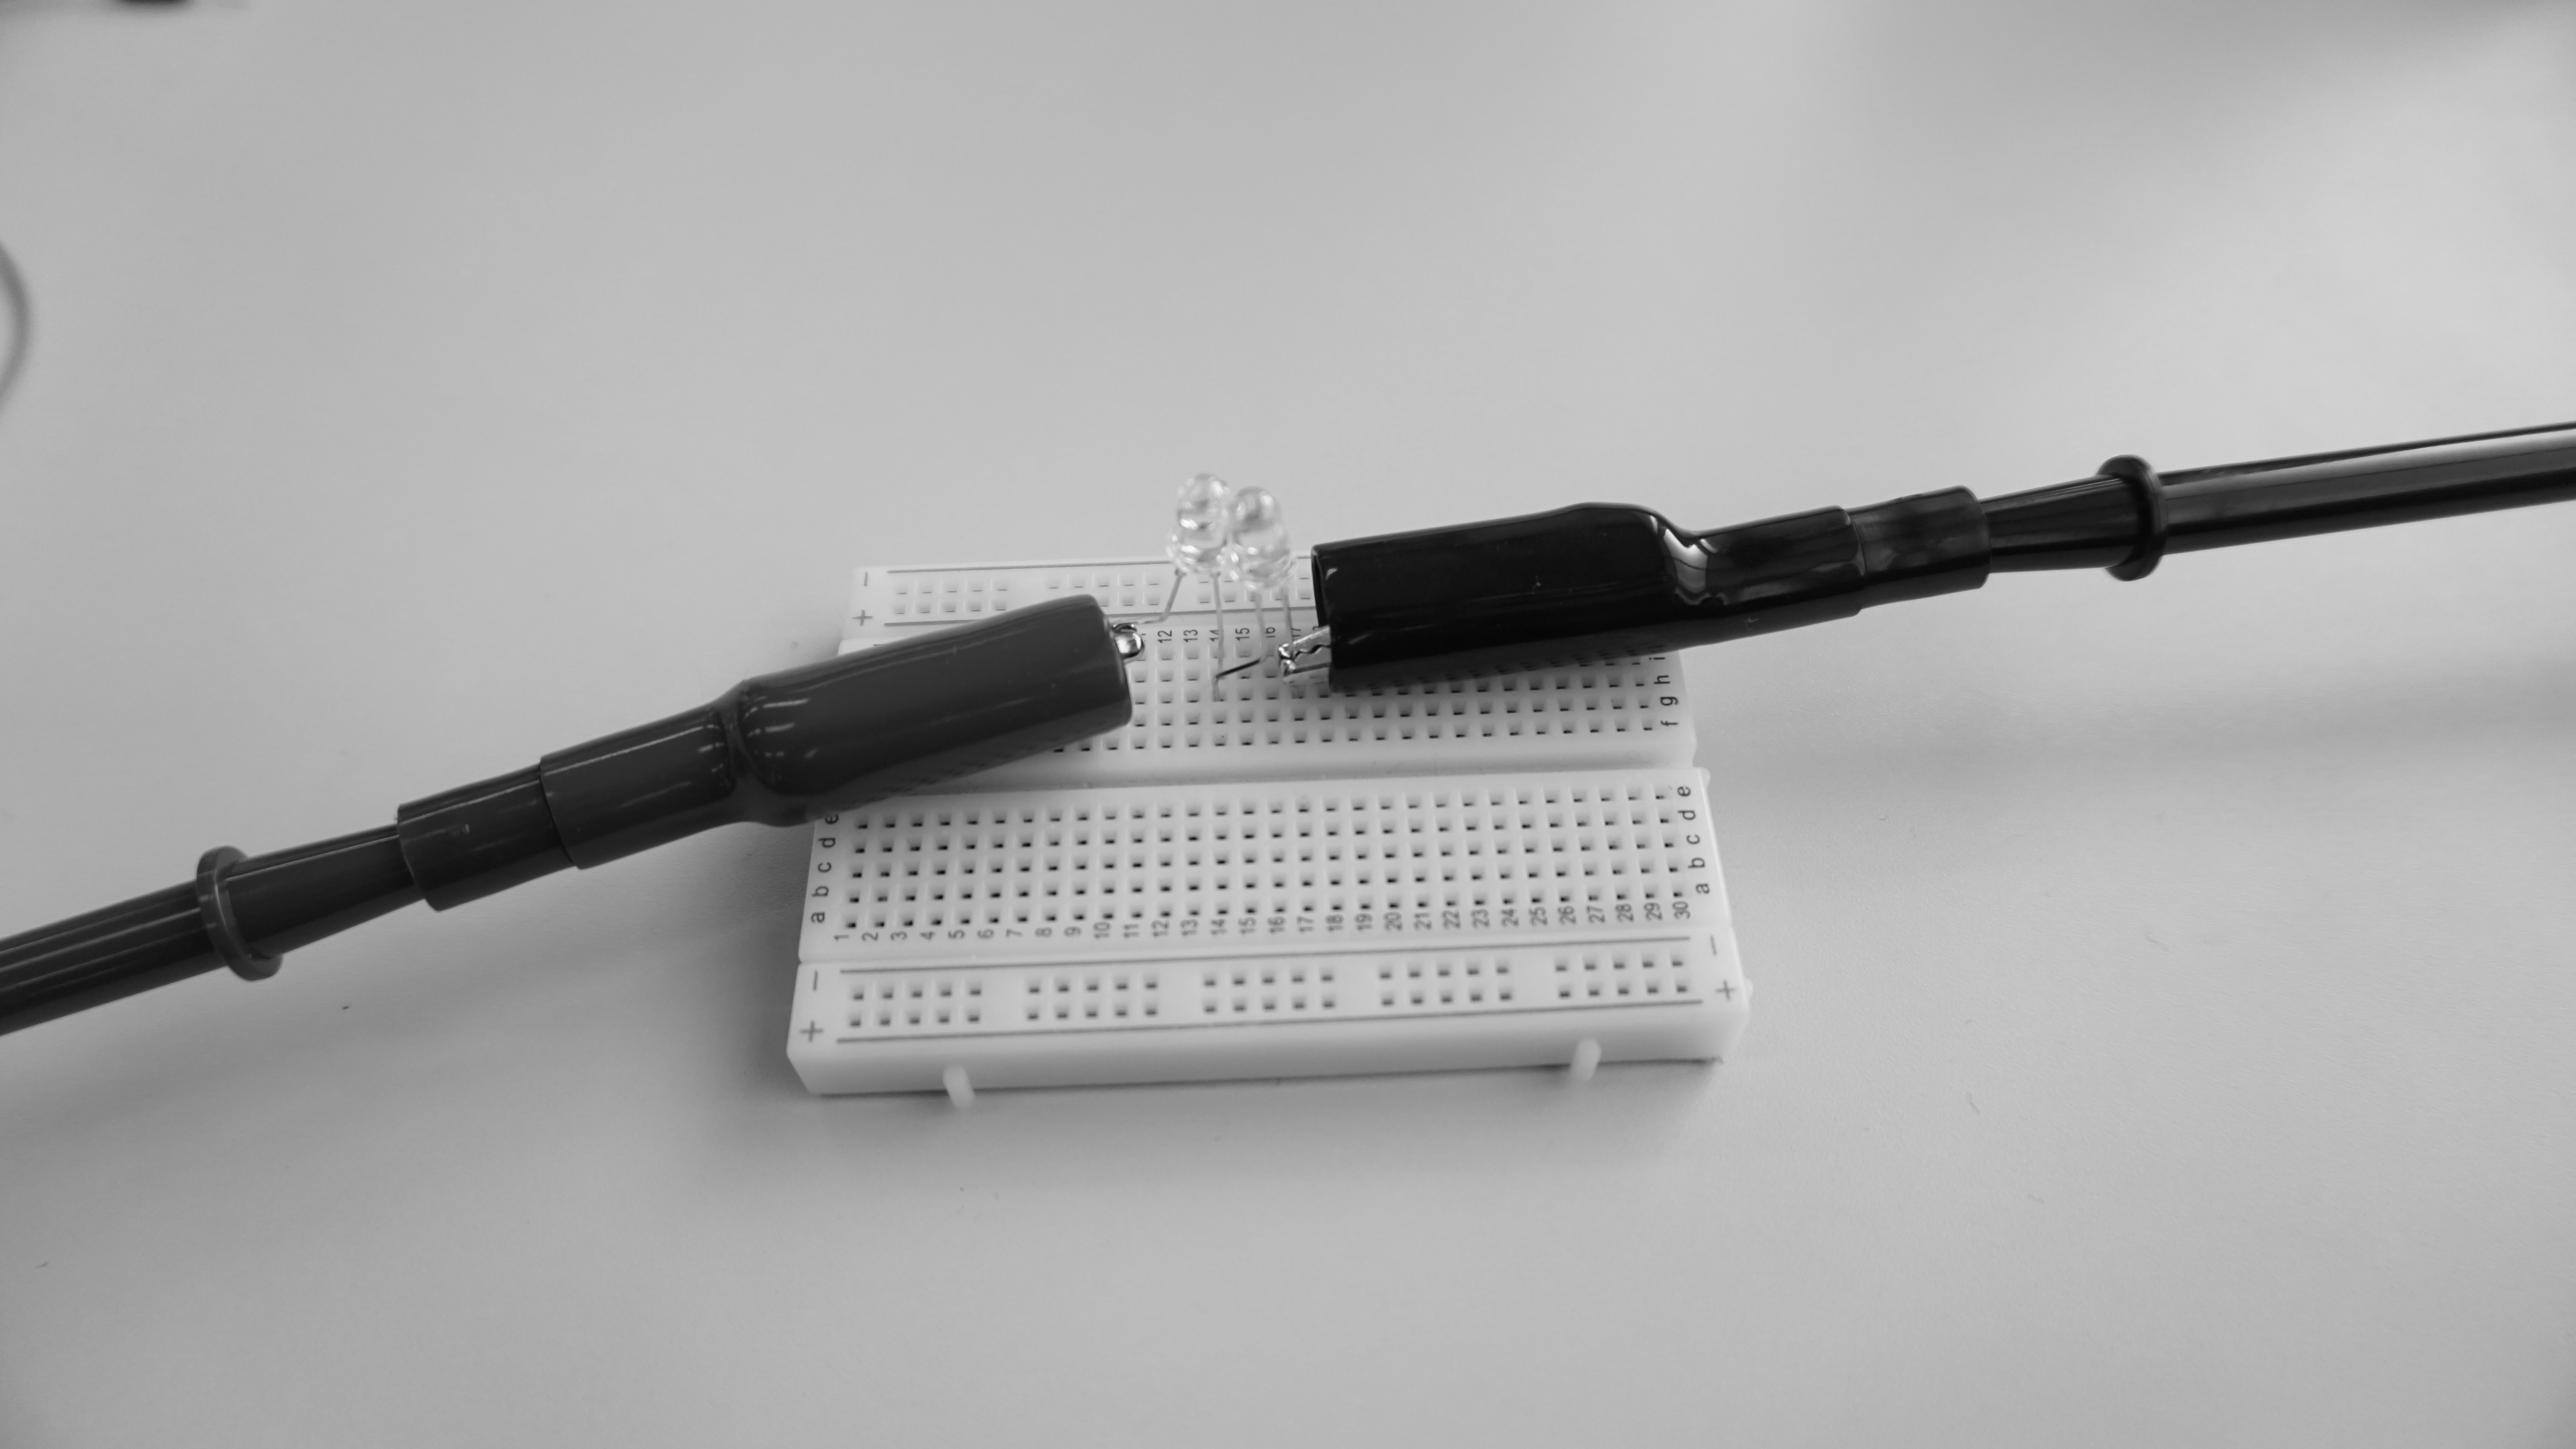
\includegraphics[width=60mm]{./assets/mouse/gray/12.JPG}
    \caption{LED2個で電流と電圧を測定している様子}
    \label{fig:led2}
\end{figure}

次に図\ref{fig:led10}のようにLED10個を直列に接続し、同じくその両端をテスターで見てみました。
その結果、約110$\mu\si\ampere$,約0.5$\si\volt$発生しました。
LED2個の時と比べて電圧が極端に小さくなっていることがわかります。
これはおそらく、LEDの電圧降下の影響をもろに受けてしまったためだと思います。
電流値は、なんかいい感じです。


\begin{figure}[htbp]
    \centering
    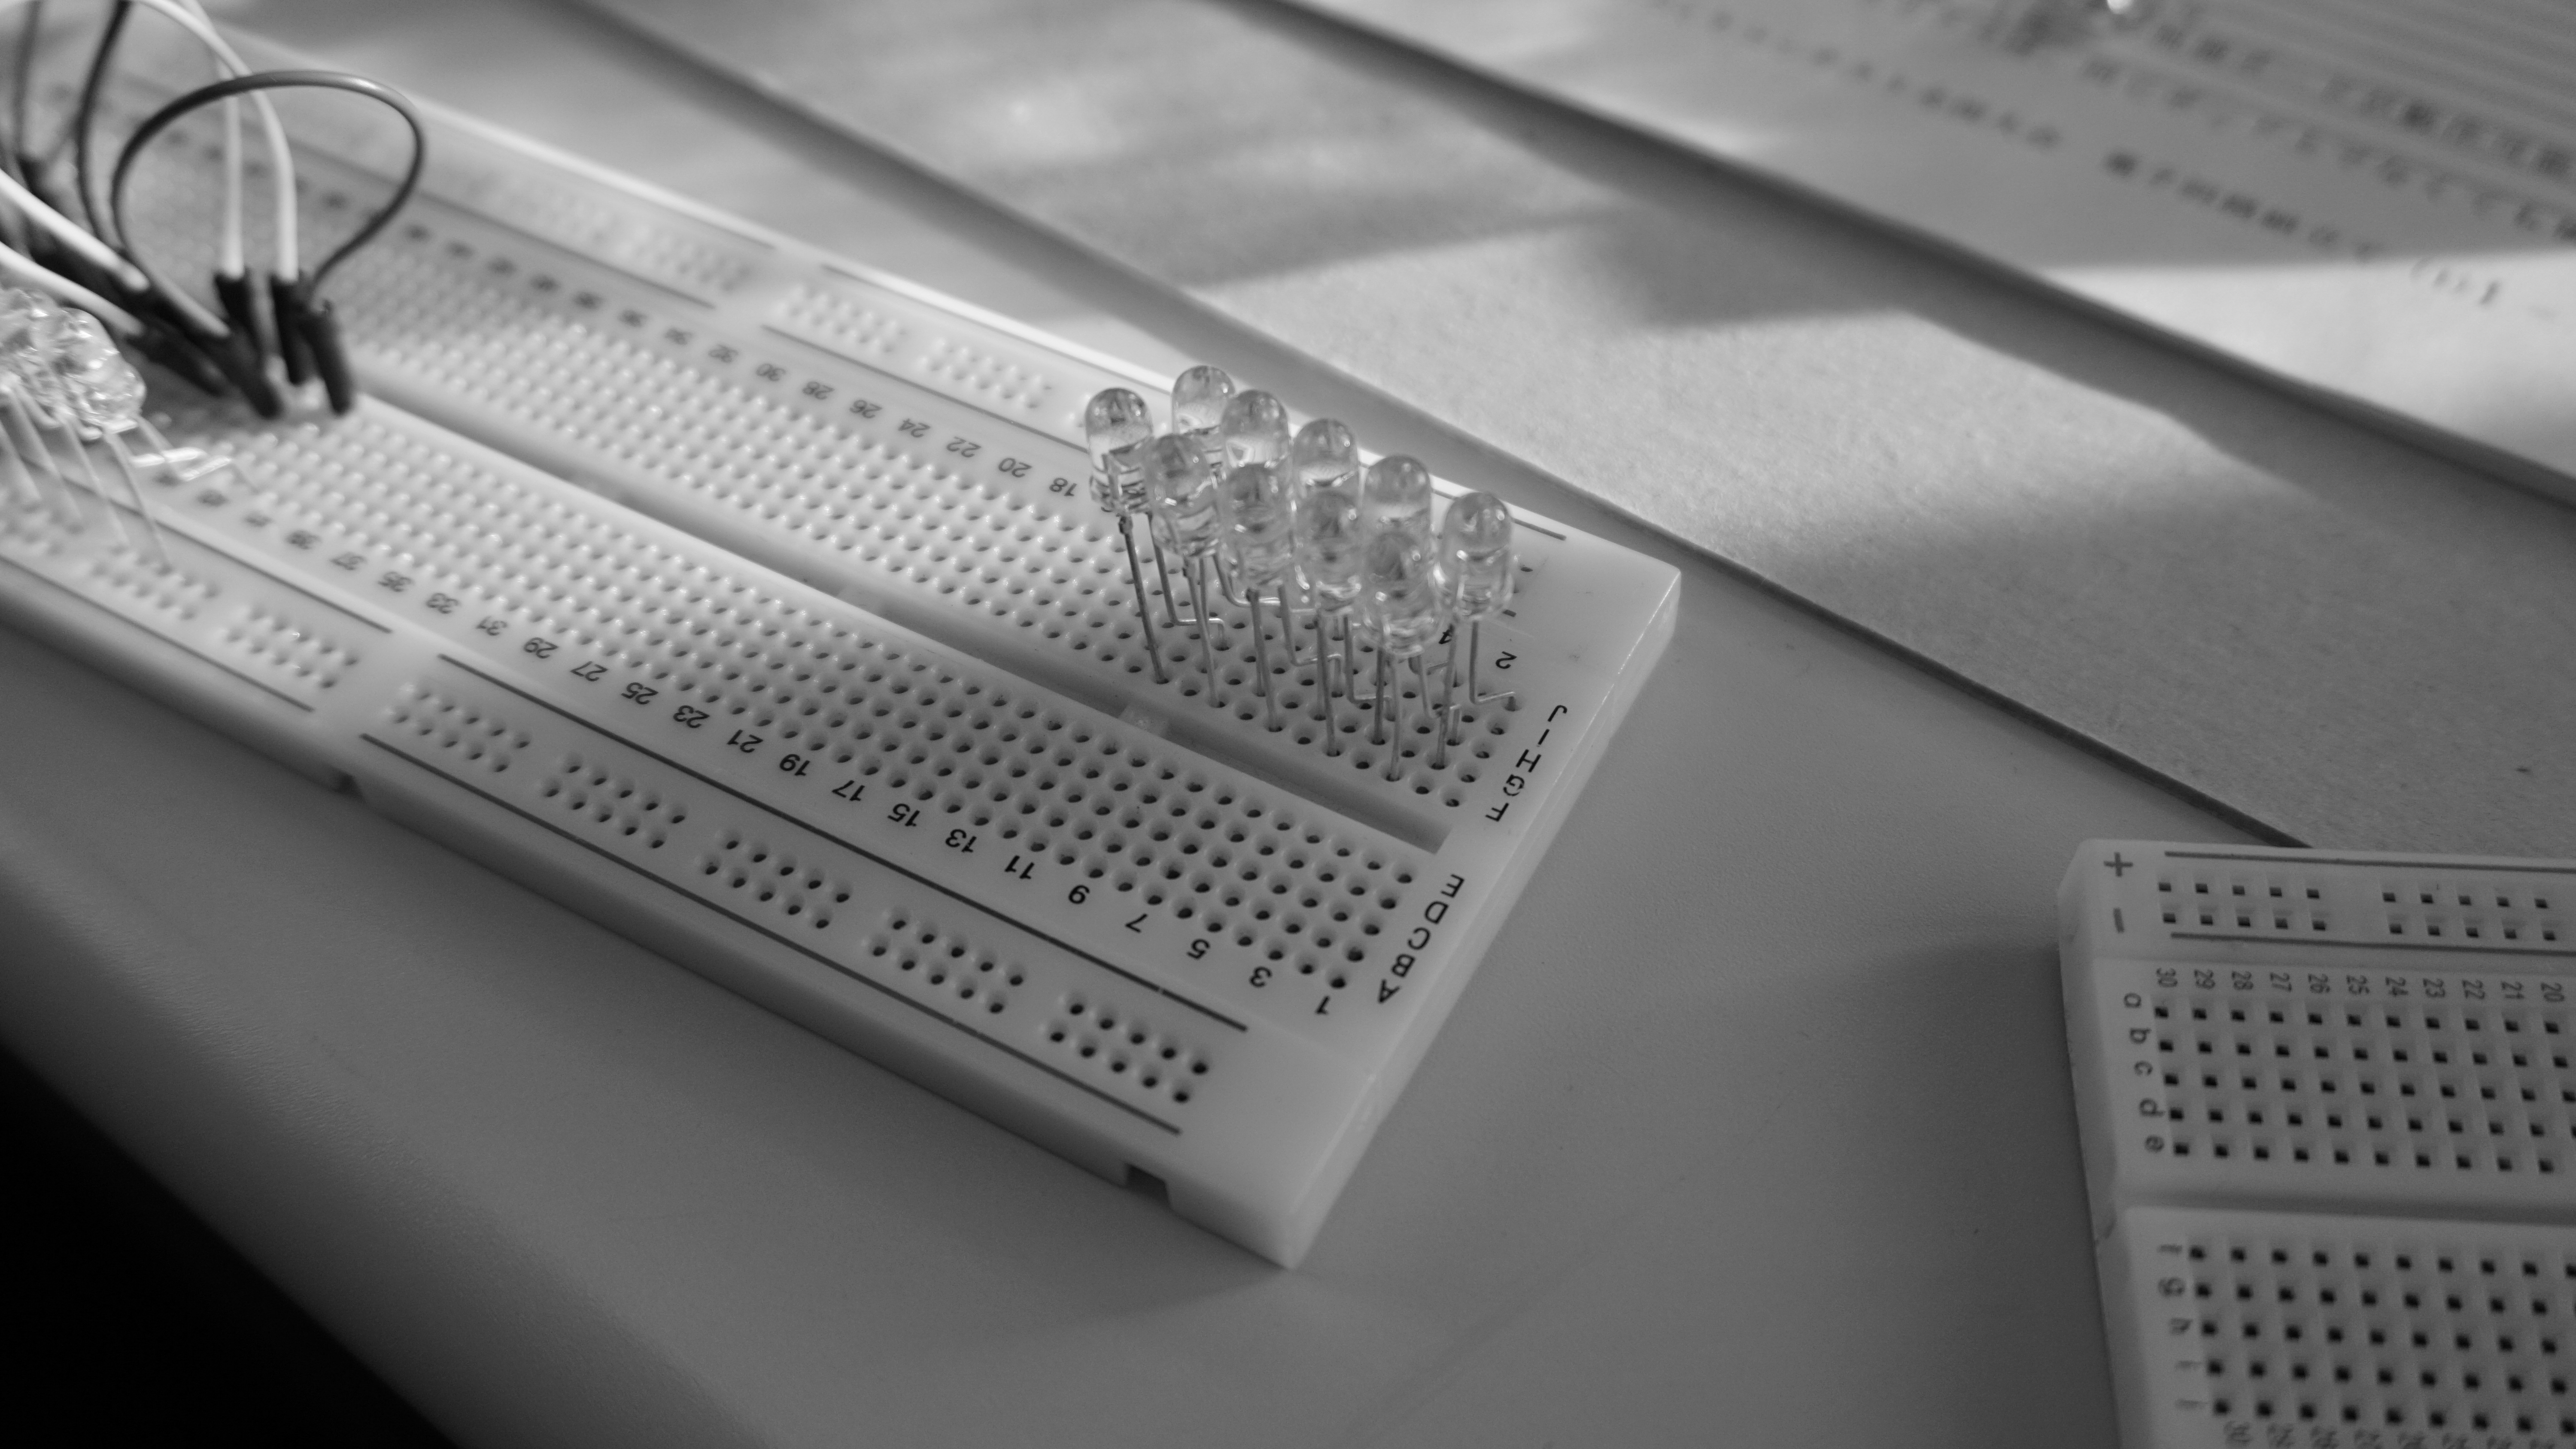
\includegraphics[width=60mm]{./assets/mouse/gray/4.JPG}
    \caption{10個のLEDを接続しているブレッドボード}
    \label{fig:led10}
\end{figure}

図\ref{fig:led_par}のようにLED2個を並列に接続し、同じくテスターで見ていきます。
こちらも太陽光で、同じ時間帯に実験しました。
並列接続の場合、約100$\mu\si\ampere$,1.5$\si\volt$発生しました。


\begin{figure}[htbp]
    \centering
    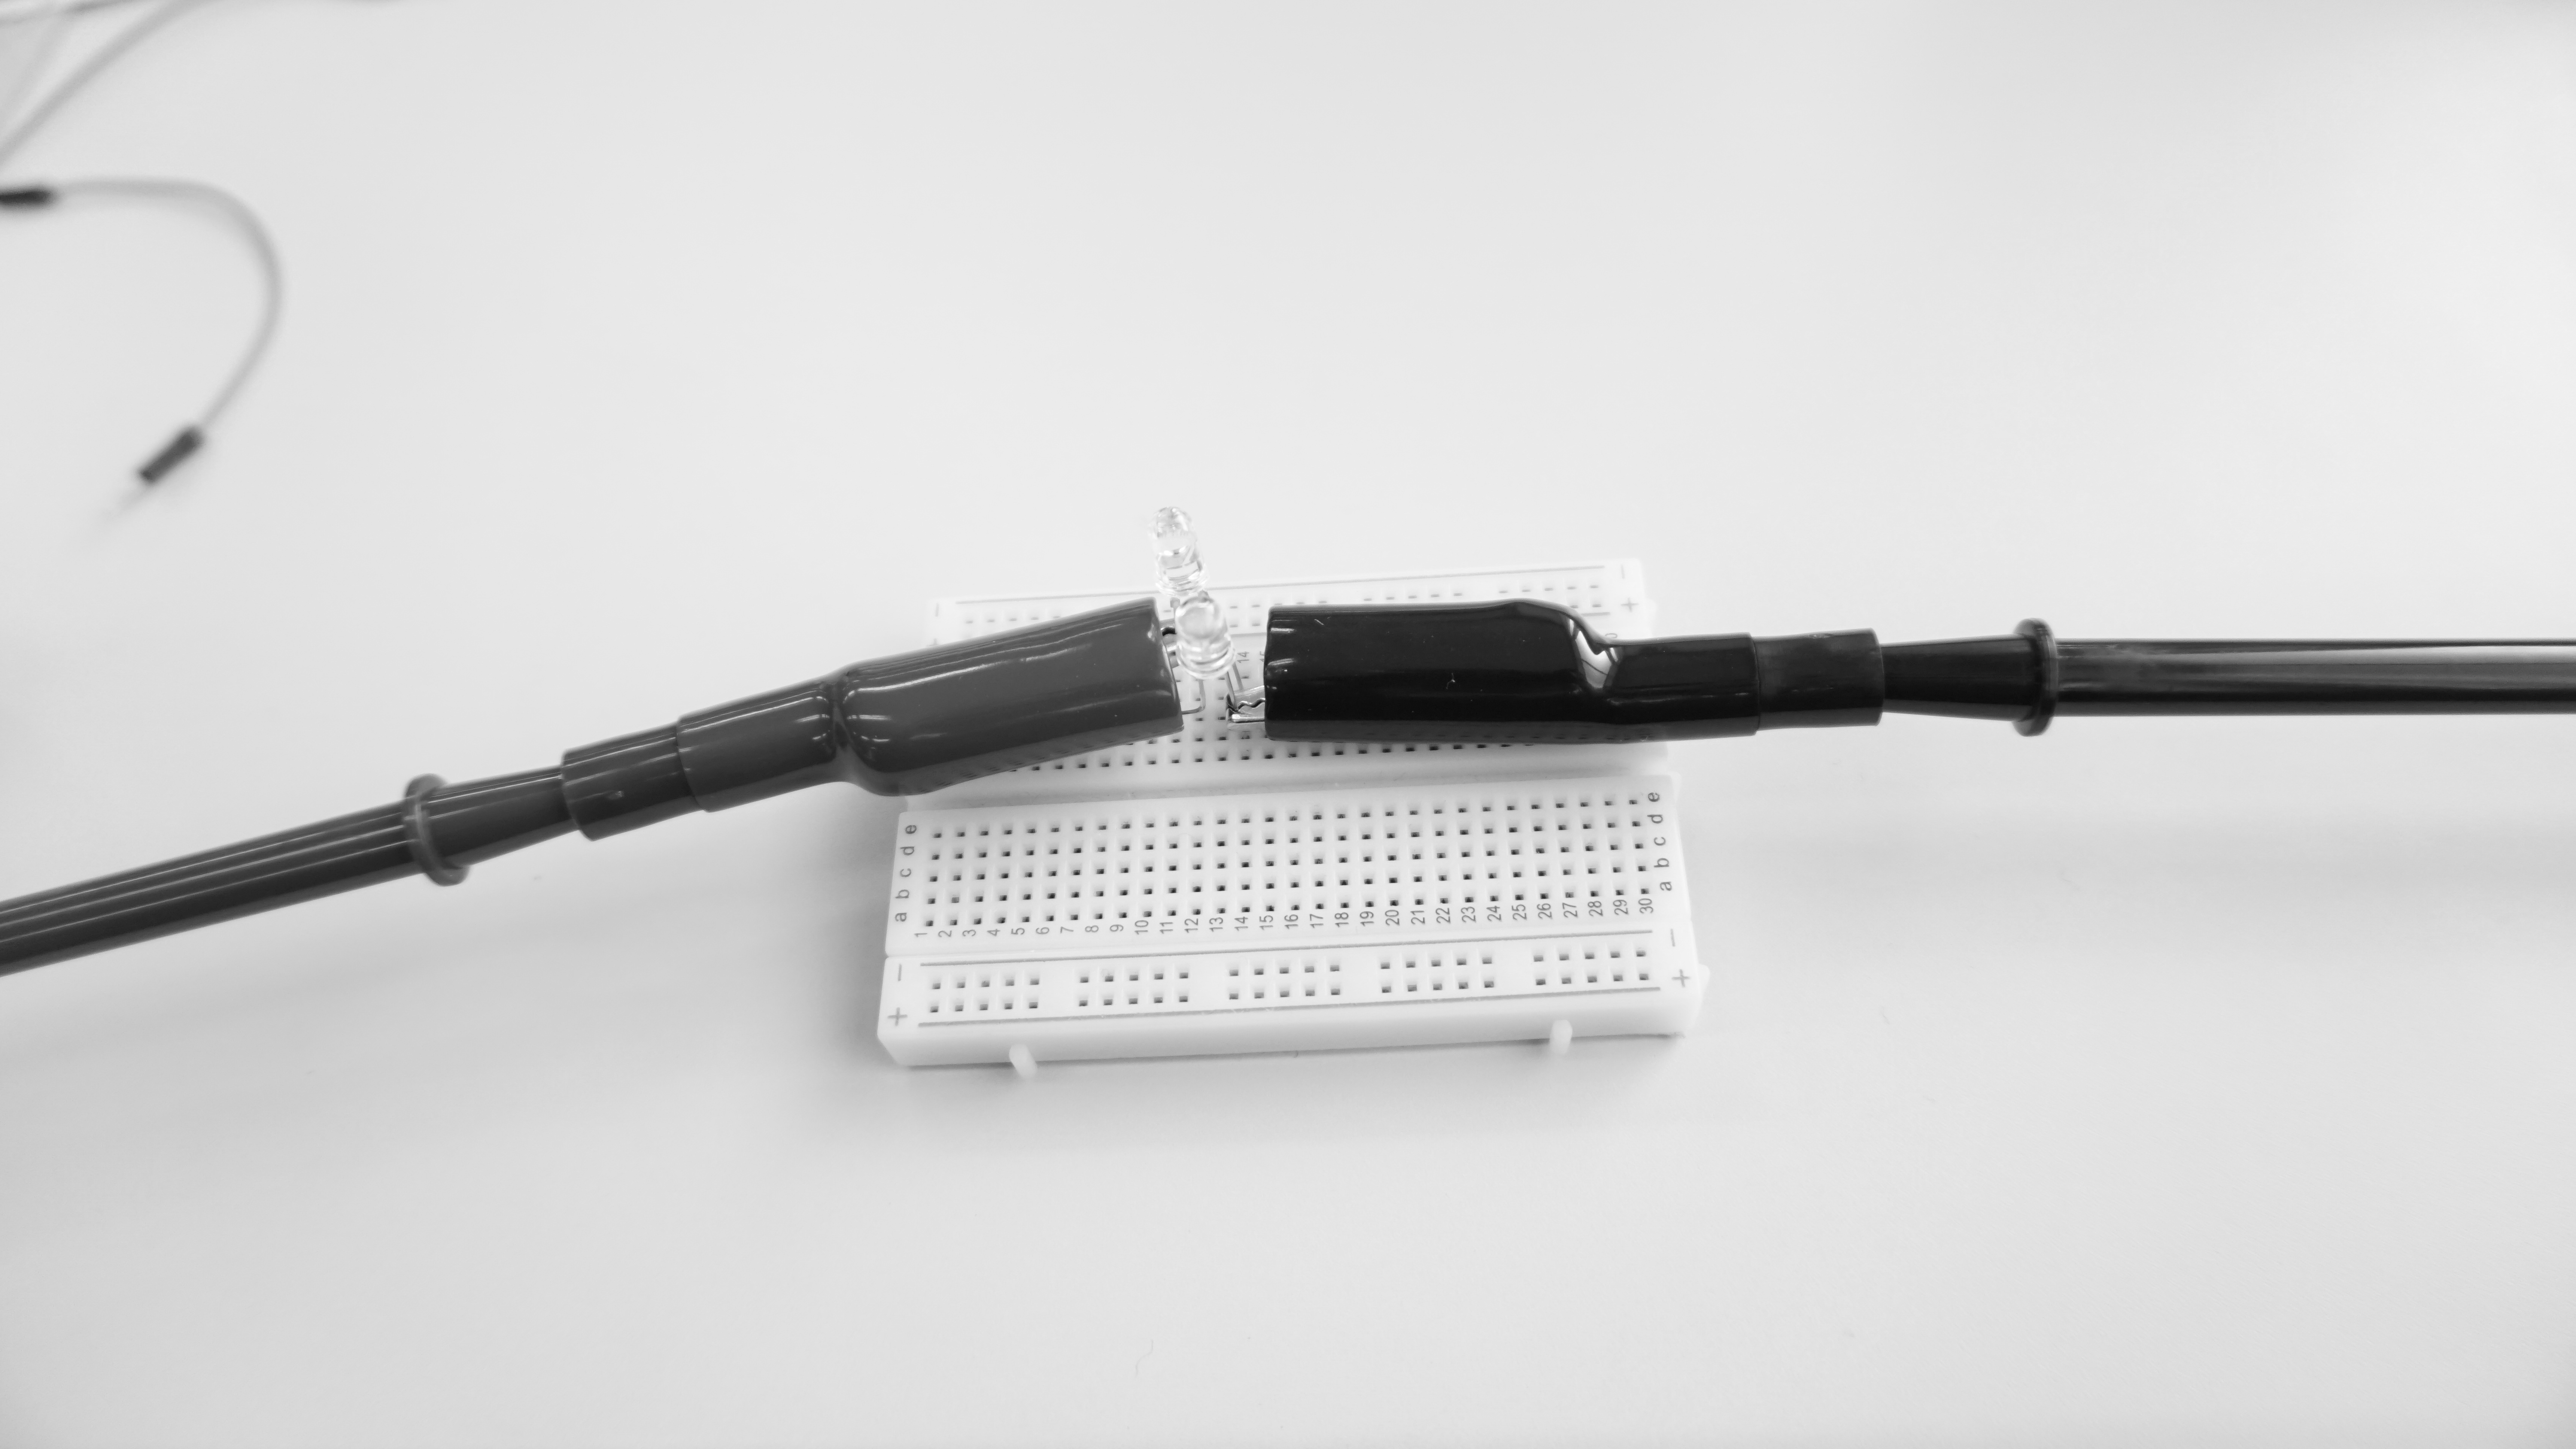
\includegraphics[width=60mm]{./assets/mouse/gray/13.JPG}
    \caption{並列接続したLEDの電流と電圧を測定している様子}
    \label{fig:led_par}
\end{figure}


先ほどと同じく、図\ref{fig:led_par10}のようにLED10個を並列に並べたものの値を取っていきます。
こちらも同じく太陽光で、同じ時間帯です。
この環境で約0.4\si{\milli\ampere},1.5$\si\volt$発生しました。やっと現実味のある数値になってきました。
これは直列と違い抵抗が並列に接続されているためだと思われます。
よくわからないけどいきなり電流が大きくなりました。


\begin{figure}[htbp]
    \centering
    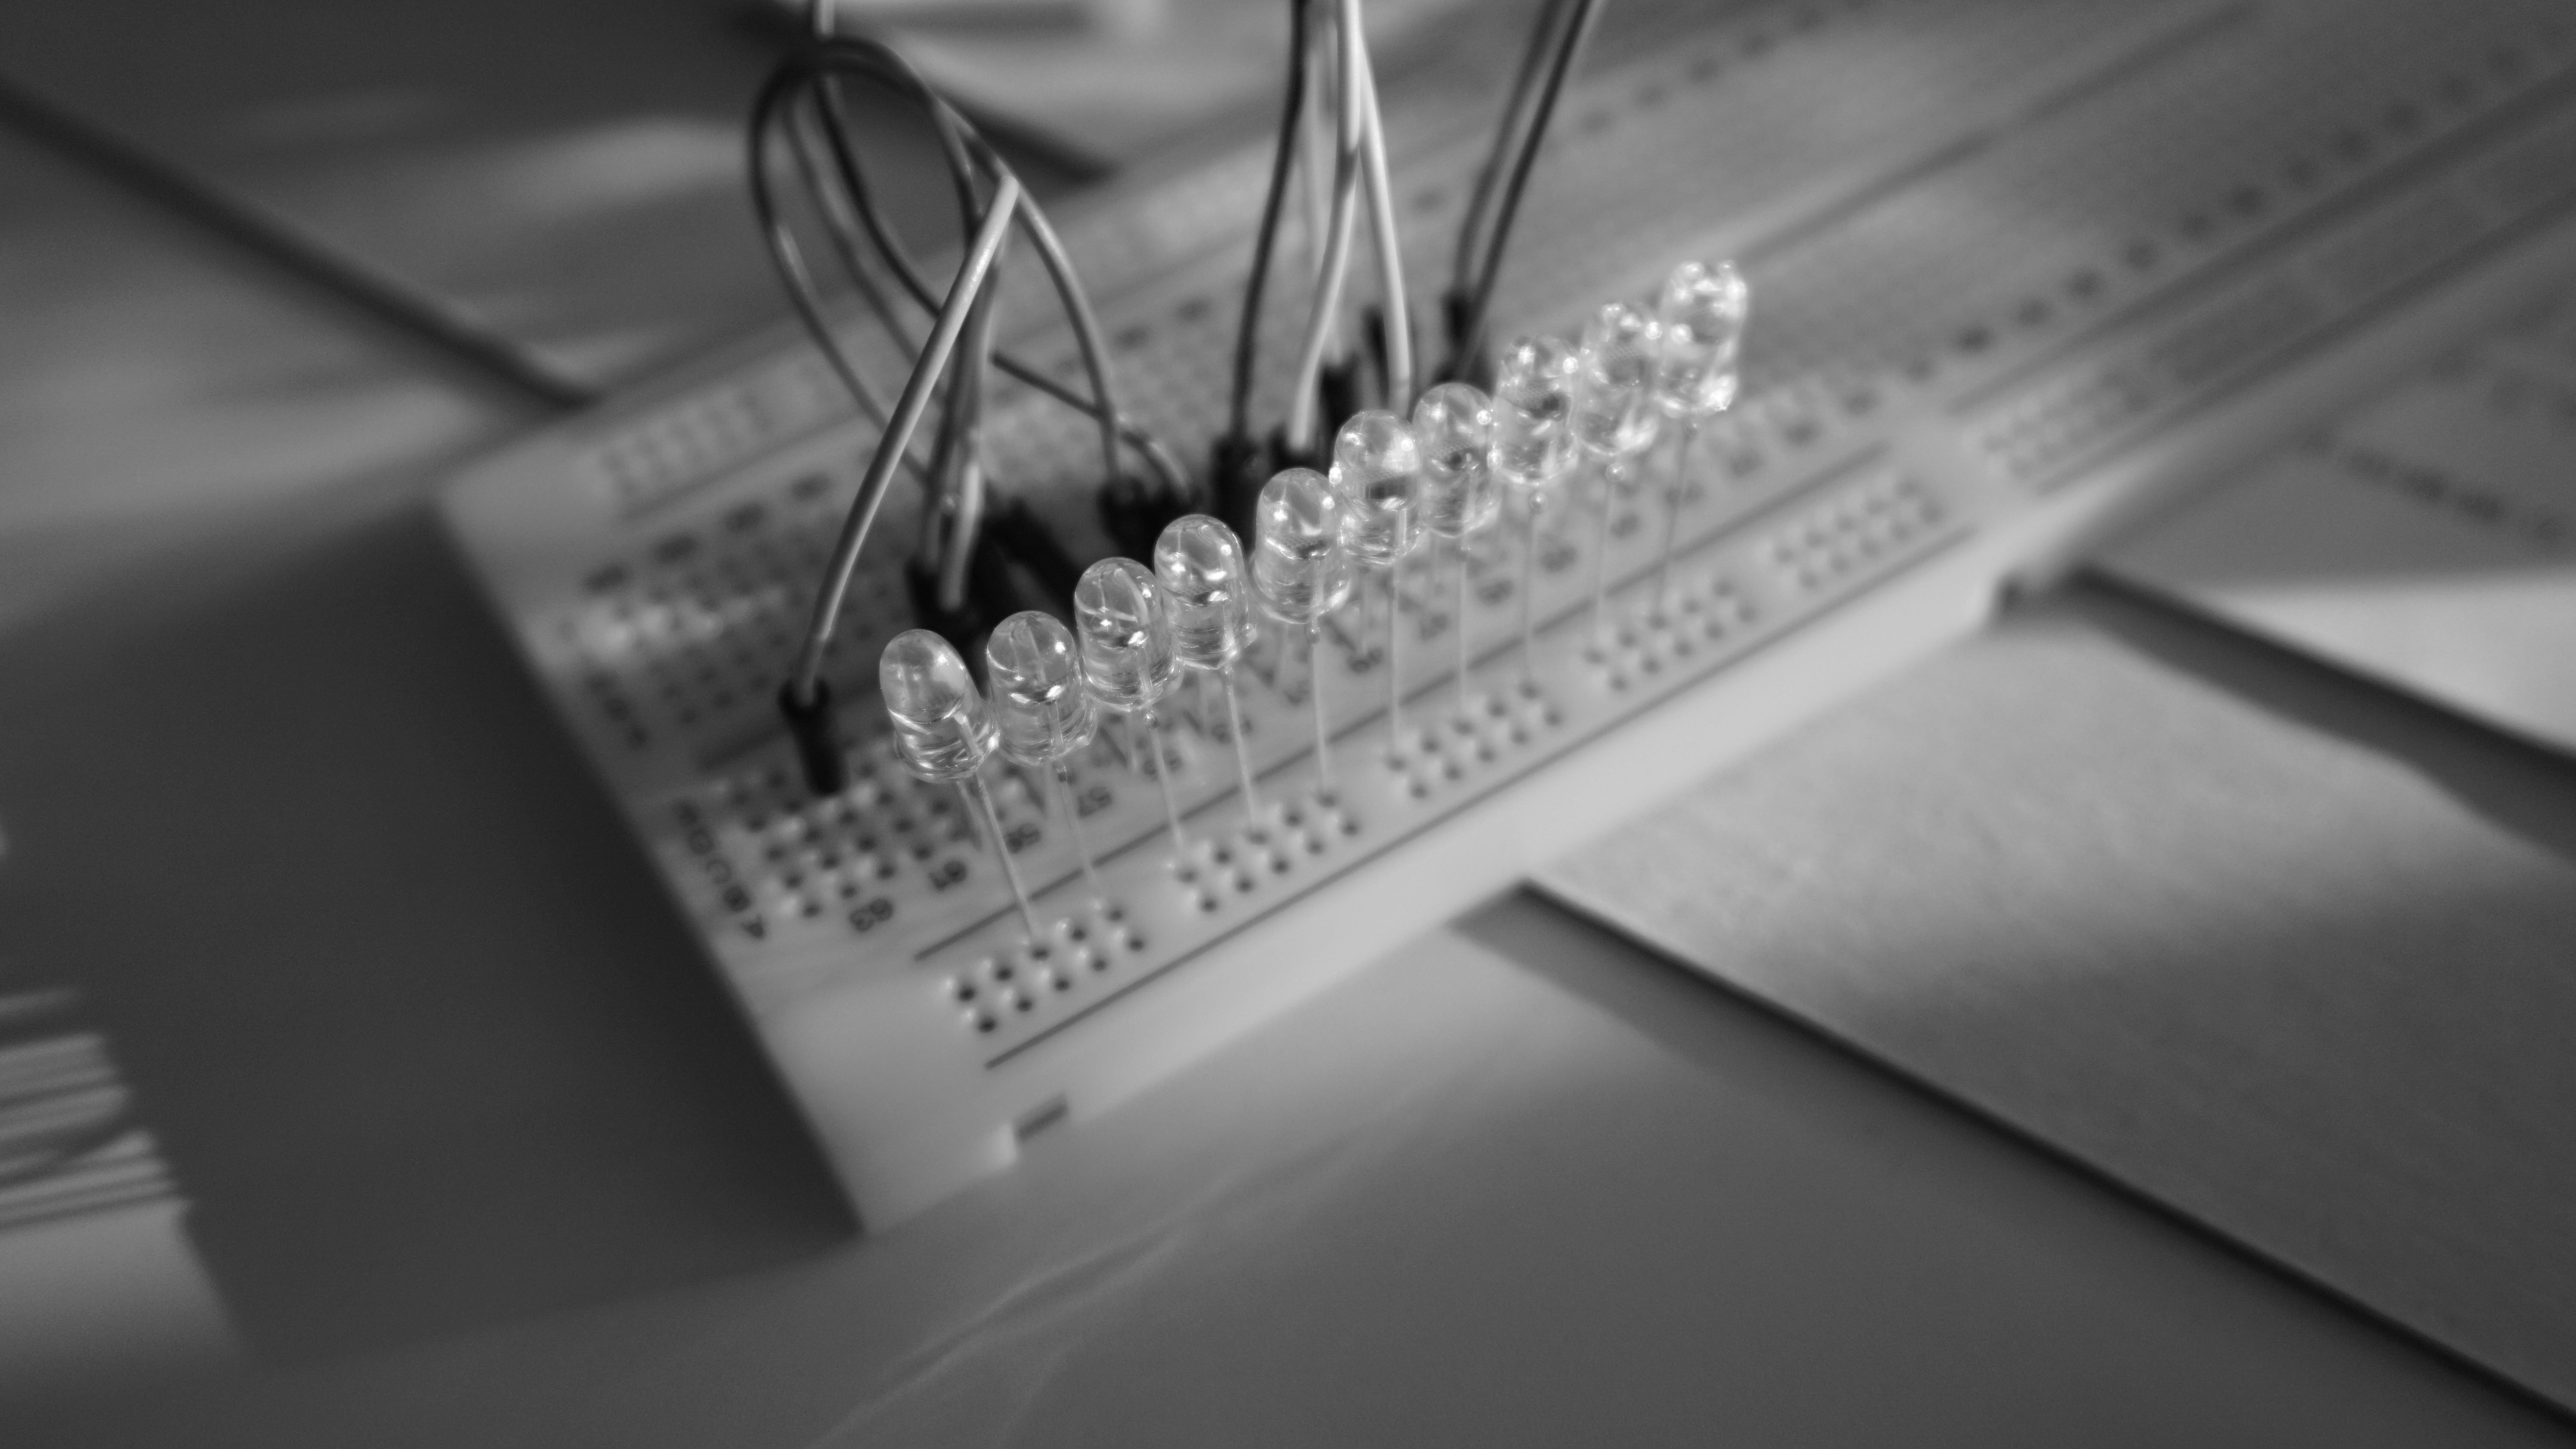
\includegraphics[width=60mm]{./assets/mouse/gray/5.JPG}
    \caption{LED10個を並列接続しているブレッドボード}
    \label{fig:led_par10}
\end{figure}

直流と並列だと並列のほうが優秀だった
並列がなんでこうなったのかはよくわからないです。
とりあえず並列でのほうがLEDを光らせるのには現実的な発電量なので、

\subsection{LEDを30個並べる}

先ほど取れたデータからだと、
LEDを30個並列に並べると1.2\si{\milli\ampere}発生するはずです。
他の実験と同じ日に行いたかったのですが、太陽が沈んでしまったので別の日に実験しました。

\begin{description}
  \item[場所]{ちかくの駐車場}
  \item[時刻]{14:30}
  \item[光源]{太陽光}
  \item[照度]{はかりわすれた}
\end{description}


\begin{figure}[htbp]
    \centering
    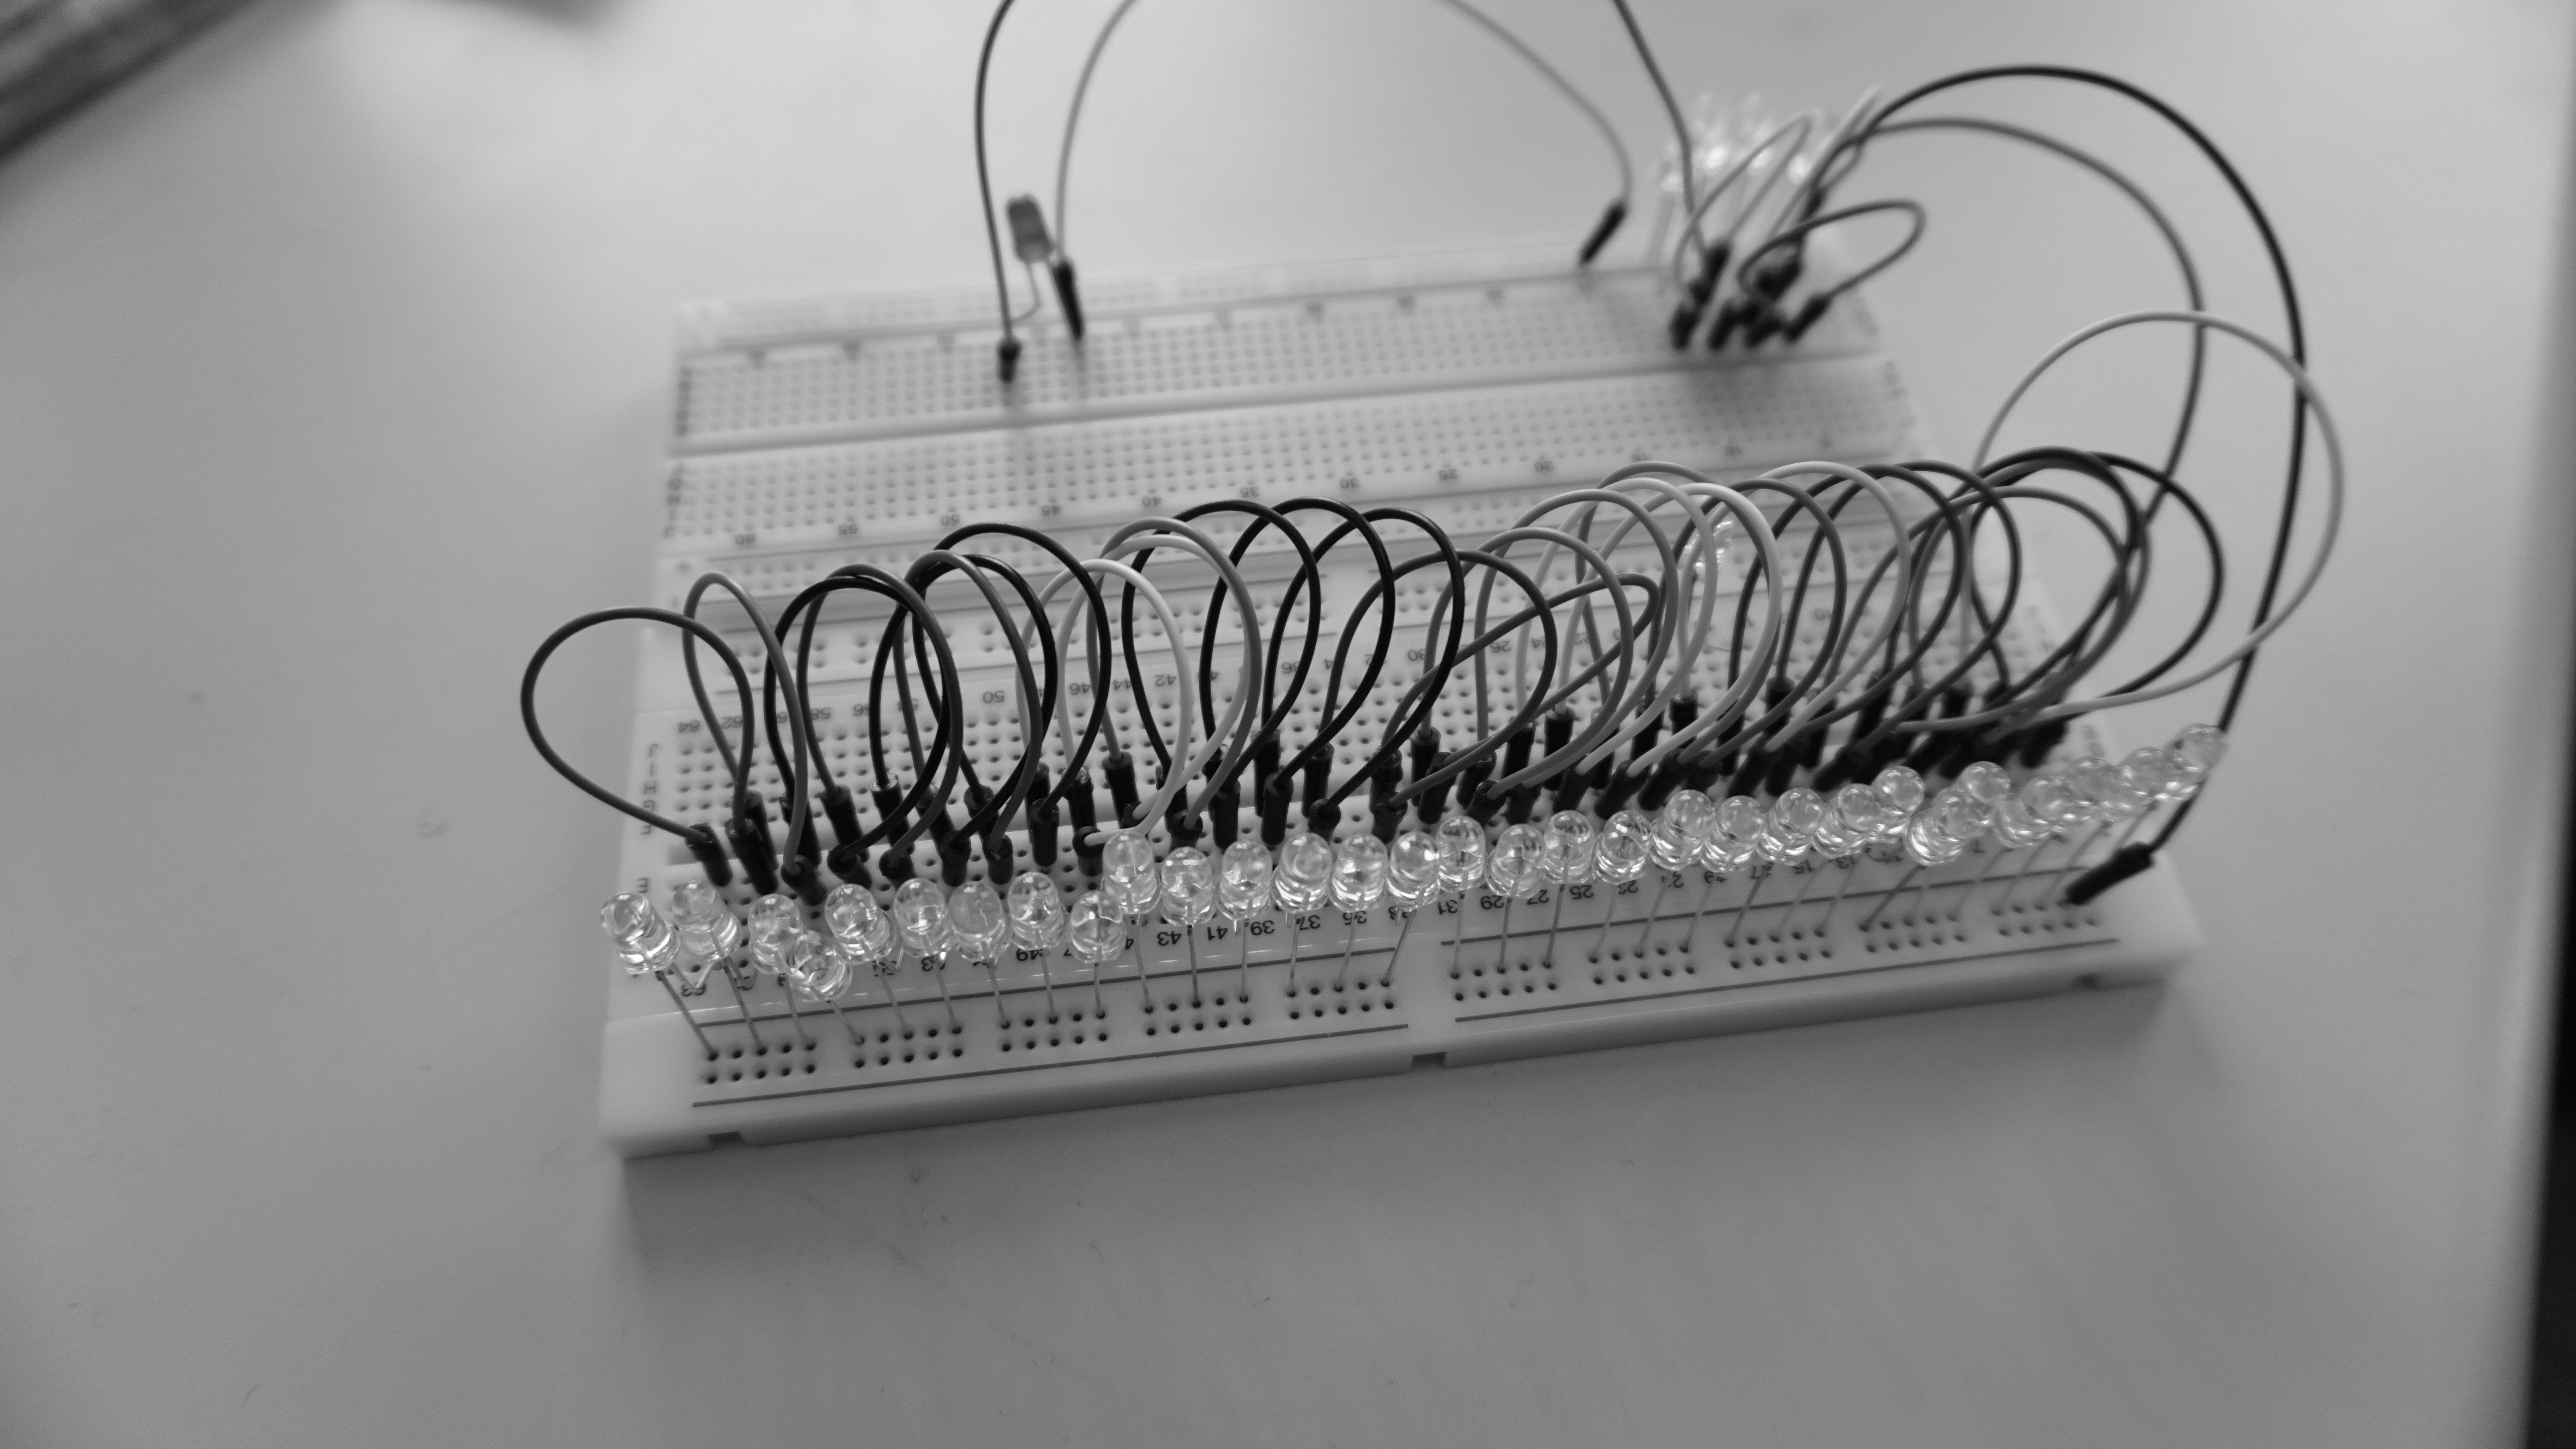
\includegraphics[width=60mm]{./assets/mouse/gray/10.JPG}
    \caption{LEDを30個並べた様子}
    \label{fig:led_par30}
\end{figure}

図\ref{fig:led_par30}のブレッドボードを駐車場へ持って行き太陽の方へLEDを向けました。
このときは、約1\si{\milli\ampere},1.5$\si\volt$となりました。
1\si{\milli\ampere}とはさわると少しぴりぴりするかしないか程度です。また、漏電も1\si{\milli\ampere}以下が許容範囲です。つまり30個並列に並べて発生した電流は漏電にもならないのです。
悲しいですね。

\subsection{波長特性}
LEDにも波長特性はあります。
なので、LEDの色によって発電量も変わってきますし、光源の波長特性によっても全然違います。
場所、光源、LEDをしっかり選ぶとより良い発電ができるかもしれません。
今度検証してみます。

\section{最後に}
LEDで発電するのはあまりお勧めできません。
まともに使おうとしたらたくさん並べなければいけないので、とてもめんどくさいです。
だけど僕はLEDで発電することに喜びを感じているので、これからもLEDで発電していこうとおもいます。


\chapterauthor{けんつ}
\chapter{入門Linux Kernel}
\section{はじめに}

最近の開発、主にその開発環境やインフラレイヤーにおいて無くてはならないものとしてDockerが挙げられる。そして、Dockerを使ってWebサービスのインフラ等を構築する場合よく利用するのはdocker-composeだろう。
この章ではDockerの基本的な部分から紹介し、docker-composeの裏側を解説したあとにDocker Remote APIを使って自分でコンテナを制御するということについて紹介する。


\section{Dockerとは}

Dockerそのものに関しては公式ドキュメントよりもさくらインターネットさんの「さくらのナレッジ Docker入門(第一回)~Dockerとは何か、何が良いのか~」で簡単に紹介されていたのでそちらを引用する。
Dockerとはその記事で次のように紹介されている。\cite{sakura}

\begin{quote}
Dockerは、インフラ関係やDevOps界隈で注目されている技術の一つで、Docker社が開発している、コンテナ型の仮想環境を作成、配布、実行するためのプラットフォームです。
(https://www.docker.com/what-docker)

Dockerは、Linuxのコンテナ技術を使ったもので、よく仮想マシンと比較されます。VirtualBoxなどの仮想マシンでは、ホストマシン上でハイパーバイザを利用しゲストOSを動かし、その上でミドルウェアなどを動かします。それに対し、コンテナはホストマシンのカーネルを利用し、プロセスやユーザなどを隔離することで、あたかも別のマシンが動いているかのように動かすことができます。そのため、軽量で高速に起動、停止などが可能です。
\end{quote}

これが全てとなる。Dockerコンテナを利用することで特にWebサービス開発の開発環境において共通のインフラをチーム全員で共有することができるなどの様々なメリットがある。


\subsection{Dockerのアーキテクチャ}
Dockerとはコンテナの色々に関わるプラットフォームを指しているが実際にコンテナを利用する場合にはdockerコマンドを通して使う場合が多い。
dockerコマンドは何をしているかというと、docker remote apiを呼び出している。このdocker remote apiなるものは、Dockerのアーキテクチャに深く関係している。


Dockerのアーキテクチャはクライアント・サーバアーキテクチャとなっておりdockerコマンドはただのCLIツールである。
そのただのCLIツールが何をしているかというとdocker daemonが提供しているREST APIライクなDocker Remote APIをコールしているに過ぎない。


Docker Remote APIはデフォルトでunixドメインソケットを用いることで利用できるようになっている。自身で設定することでtcpによるリクエストを許可することも出来る。これ移行の章ではそれを有効にしている前提で話を進めていく。

\section{Docker Composeとは}

Docker-Composeとは、前述のDockerコンテナを複数利用する場合にそれらをまとめて管理するためのツールである。
Dockerコマンドだけでは何が問題かというと、例えばweb開発においてインフラをDockerコンテナで用意するならばNginxのコンテナにMySQLのコンテナ、PHPやRailsが動作するコンテナなど複数のコンテナが必要になってくる。
これら全てをdocker runで呼び出すとシェルなどにまとめておく必要がある。そして利便性に欠ける。では、サービスに必要なコンテナ群を一箇所でまとめて管理してしまいたい。そういう場合にdocker-composeを利用するのは非常に有効な手段となる。


そして、Docker ComposeはDocker Remote APIを通してdocker-compose.ymlに記載されているコンテナ群を管理している。
この点がこれ移行の説明で非常に重要になっていく。

\section{docker-composeを自作する}

ここまで紹介した情報を元にこの章の本題である、Dockerコンテナの制御を行う。制御といっても何をするかというとDocker Remote APIを使って超絶最高にシンプルなdocker-composeを作ってみる。Golangで。書いたことあまりないけど。


それではまず要件を以下に定義する。
\begin{itemize}
    \item ymlを解析して作成するコンテナやボリューム、ポートを設定できる
    \item コンテナを走らせる。
    \item コンテナを落とす。
    \item 起動しているコンテナのステータスを取る
\end{itemize}

\subsection{コマンドライン引数をパースする}

まずは、cliツールを作る上でコマンドライン引数をパースする必要がある。そこで import flag を使って簡易的にパースしていく。今回のcliツールではup,down,statusまでできれば十分なのでそれだけ定義する。

\begin{minted}[frame=lines,framesep=2mm,baselinestretch=1.2,fontsize=\footnotesize,linenos,breaklines]{go}
package main

import (
    "flag"
    "fmt"
)

func main() {
    flag.Parse()

    switch flag.Arg(0) {

    case "up":
        fmt.Println("up")
    case "down":
        fmt.Println("down")
    case "status":
        fmt.Println("status")
    default:
        fmt.Println("unknown")
    }
}
\end{minted}

\subsection{ymlをパースする}

次にそれなりに重要な機能であるymlのパースを行う。ただパーサーから書いている時間はなかったのでここでは gopkg.in/yaml.v2 というパッケージを使用する。

\begin{minted}[frame=lines,framesep=2mm,baselinestretch=1.2,fontsize=\footnotesize,linenos,breaklines]{go}
package main

import (
    "flag"
    "fmt"
    yaml "gopkg.in/yaml.v2"
    "io/ioutil"
)

type Services struct {
    Services []Docker `yaml:"services"`
}

type Docker struct {
    Name string     `yaml:"name"`
    Image string    `yaml:"image"`
    Command string  `yaml:"command"`
}

func main() {

    buf, err := ioutil.ReadFile("./lite-compose.yml")
    if err != nil {
        panic(err)
    }

    var parsed Services
    err = yaml.Unmarshal(buf, &parsed)
    if err != nil {
        panic(err)
    }

    fmt.Println(parsed)

    flag.Parse()
    switch flag.Arg(0) {

    case "up":
        fmt.Println("up")
    case "down":
        fmt.Println("down")
    case "status":
        fmt.Println("status")
    default:
        fmt.Println("unknown")
    }
}
\end{minted}

コード自体はこれでいいのだがひとつ問題がある。docker-composeのようなパターンのymlを今回使ったライブラリではパースできないことだ。
しかし、パーサーから探すのはめんどくさいので仕方なくymlの形式を以下のようにして lite-compose.yml とする。

\begin{minted}[frame=lines,framesep=2mm,baselinestretch=1.2,fontsize=\footnotesize,linenos,breaklines]{yaml}

services:
-
  name: ubuntu
  image: ubuntu
  command: 'echo "hello, world"'

\end{minted}

これを実行すると構造体として表示される。ただこれだけでは色々と不十分なのでエラーハンドリングを追加してファイルを分割してみた。

\begin{minted}[frame=lines,framesep=2mm,baselinestretch=1.2,fontsize=\footnotesize,linenos,breaklines]{go}
package main

import (
    "flag"
    "fmt"
    "gopkg.in/yaml.v2"
    "io/ioutil"
)

func main() {

    buf, err := ioutil.ReadFile("./lite-compose.yml")
    if err != nil {
        panic(err)
    }

    var parsed Services
    err = yaml.Unmarshal(buf, &parsed)
    if err != nil {
        panic(err)
    }

    if err := requireNotExist(); !parsed.validate() {
        panic(err)
    }

    flag.Parse()
    switch flag.Arg(0) {

    case "up":
        fmt.Println("up")
    case "down":
        fmt.Println("down")
    case "status":
        fmt.Println("status")
    default:
        fmt.Println("unknown")
    }
}
\end{minted}

\begin{minted}[frame=lines,framesep=2mm,baselinestretch=1.2,fontsize=\footnotesize,linenos,breaklines]{go}
package main

import "errors"

type Services struct {
    Services []Docker `yaml:"services"`
}

type Docker struct {
    Name string     `yaml:"name"`
    Image string    `yaml:"image"`
    Command string  `yaml:"command"`
}

func (services *Services) validate() bool {
    for _, docker := range services.Services {
        if docker.Image == "" || docker.Name == "" {
            return false
        }
    }
    return true
}


func requireNotExist() error {
    return errors.New("The syntax of yaml is incorrect")
}
\end{minted}

\section{コンテナを制御する}

ここまでやってきたら後はdocker remote apiを使ってdockerコンテナを立ち上げ落としてステータスを取れるようにする。
docker remote api自体はunixドメインソケットかtcpまたはhttpでリクエストを飛ばすことで利用することができる。ここではそれらを順を追って説明していく。
本来はそれらリクエスト部分を自作するつもりであったが今回は golang でdocker remote apiを利用できるライブラリのgithub.com/docker/dockerを使用する。


実際にdocker remote apiを使ったコンテナ制御は以下のようになる。
\begin{minted}[frame=lines,framesep=2mm,baselinestretch=1.2,fontsize=\footnotesize,linenos,breaklines]{go}
package main

import (
    "context"
    "fmt"
    "github.com/docker/docker/api/types"
    "github.com/docker/docker/api/types/container"
    "github.com/docker/docker/api/types/network"
    "github.com/docker/docker/client"
    "os"
    "strings"
    "time"
)

func createContainer(services Services) {
    ctx := context.Background()
    cli, err := client.NewClientWithOpts(client.WithVersion("1.39"))
    if err != nil {
        panic(err)
    }

    p, _ := os.Getwd()
    split := strings.Split(p, "/")
    current := split[len(split)-1]

    for _, service := range services.Services {

        hostConfig := &container.HostConfig{}
        containerConfig := &container.Config{
            Image: service.Name,
            Tty: true,
            Cmd: strings.Split(service.Command, " "),
        }
        networkConfig := &network.NetworkingConfig{}

        resp, err := cli.ContainerCreate(ctx, containerConfig, hostConfig, networkConfig, current+"_"+service.Name)
        if err != nil {
            fmt.Println(err)
        } else {
            err := cli.ContainerStart(ctx, resp.ID, types.ContainerStartOptions{})
            if err != nil {
                fmt.Println(err)
            } else {
                fmt.Println(resp)
            }

        }
    }
}

func killContainer(services Services) {
    ctx := context.Background()
    cli, err := client.NewClientWithOpts(client.WithVersion("1.39"))
    if err != nil {
        panic(err)
    }

    p, _ := os.Getwd()
    split := strings.Split(p, "/")
    current := split[len(split)-1]

    timeout := 5 * time.Second

    for _, service := range services.Services {
        resp := cli.ContainerStop(ctx, current+"_"+service.Name, &timeout)
        fmt.Println(resp)
    }
}

func getDockerImageList() {

    ctx := context.Background()
    cli, err := client.NewClientWithOpts(client.WithVersion("1.39"))
    if err != nil {
        panic(err)
    }

   list, err := cli.ImageList(ctx, types.ImageListOptions{})
   if err != nil {
        panic(err)
   }

   for _, image := range list {
       fmt.Printf("RepoTags: %s, Labels: %s, Container: %d, Size: %d\n", image.RepoTags, image.Labels, image.Containers, image.Size)
   }

}


func getDockerPs() {
    ctx := context.Background()
    cli, err := client.NewClientWithOpts(client.WithVersion("1.39"))
    if err != nil {
        panic(err)
    }

    containers, err := cli.ContainerList(ctx, types.ContainerListOptions{
        All: true,
    })

    if err != nil {
        panic(err)
    }

    for _, container := range containers {
        fmt.Printf("ID: %s, Name: %sm Image: %s, Command: %s\n", container.ID, container.Names, container.Image, container.Command)
    }
}
\end{minted}

ここでは、ライブラリを使用してHostConfigなどを設定し、コンテナを作成した上で起動させるという一連の流れを行っている。
さらにportsやvolumesなど今回は導入しなかったが通常docker-compose.ymlで設定するようなパラメータ群を設定することもできるので興味があれば実際に試して欲しい。

\section{おわりに}

ここで紹介したように、dockerとはプラットフォームであり普段使うようなdockerコマンドは実際にはdocker remote apiを叩いているに過ぎない。また、docker-composeはそれらをまとめて管理しているがこれもまたdocker remote apiを叩いているだけである。
そのため、これらを応用すれば競技プログラミングやオンライン実行環境で実際にコードを動かす部分をユーザのアクションに併せて作成することができる。
是非そのようなサービスを開発する際にここに書いてある知識を応用して貰えると締め切りの前日からこのようなものを作り始めた甲斐があるというものである。


\begin{thebibliography}{10}
    \bibitem{sakura} Docker入門(第一回)~Dockerとは何か、何が良いのか~ | さくらのナレッジ https://knowledge.sakura.ad.jp/13265/
    \bibitem{unixdomain} tcp-hist.ps http://osnet.cs.binghamton.edu/publications/TR-20070820.pdf
\end{thebibliography}


\chapterauthor{さわだ}
\chapter{自作エディタ入門編}
\section{はじめに}
皆さんはちょっとしたメモやプログラミングにどんなエディタを使いますか?Vim?それともEmacs?まぁ色々ありますよね.
人それぞれ好き嫌いがあると思います.僕はVimを自分好みに拡張するのが好きです\footnote{そこのEmacs教徒,石を投げないで!}.
でも,人には自作欲求があります.CPU,OS,言語,更に最近はキーボードなどが人気ですが,エディタも中々面白いですよ.
CUIは時代遅れなんてそんなの気にしちゃいけません.
ソースコードは\url{https://github.com/takuzoo3868/td}に置いてあります.

\section{準備}
テキストエディタと言いつつも初めから高機能なエディタを自作するのは至難の業です.
そこで,最低限ファイルを編集して保存できるようにする所から始めるといいかなと思います.
次にシンタックスハイライト対応や文字列検索機能などを考えていきましょう.
リポジトリにあるテキストエディタのファイル構造は以下ようになっています.

\begin{figure}[H]
    \dirtree{%
    .1 td/.
    .2 modules/ \dotfill  \begin{minipage}[t]{7cm}
                              拡張機能を追加していくディレクトリ{.}
    \end{minipage}.
    .3 syntax/ \dotfill  \begin{minipage}[t]{7cm}
                             シンタックスハイライト用の構造体を定義{.}
    \end{minipage}.
    .2 LICENSE.
    .2 Makefile.
    .2 README.md.
    .2 td.c \dotfill  \begin{minipage}[t]{7cm}
                              メインとなるソースコード{.}
    \end{minipage}.
    .2 td.h \dotfill  \begin{minipage}[t]{7cm}
                              定数定義や構造体を含むヘッダ{.}
    \end{minipage}.
    }
\end{figure}
外部ライブラリに依存しない事を目標としていますが,Cコンパイラと\mintinline{bash}{make}コマンドは準備する必要があります.
\mintinline{bash}{cc --version}や\mintinline{bash}{make -v}でインストールされているかどうか確認できます.
自身の環境にコンパイラがインストールされていなかった場合は,Google先生に聞いてみましょう.

\subsubsection{makeによるコンパイル}
解説のために本文中では\mintinline{bash}{hoge}と記載しますが,
好きな名前に置き換えて下さい.
\mintinline{bash}{cc hoge.c -o hoge}などと打ち込めばコンパイルできます.
しかし試行錯誤を繰り返すため,再コンパイルの度に同じ事をするのはあまりスマートではありません.
\mintinline{bash}{make}を用いることでプログラムコンパイルを少しだけ楽にしておきましょう.
\mintinline{bash}{Makefile}を作成し,以下の内容を記述しておきます.
\begin{minted}[frame=lines,framesep=2mm,baselinestretch=1.2,fontsize=\footnotesize,linenos,breaklines]{text}
hoge: hoge.c
$(CC) -o hoge hoge.c -Wall -W -pedantic -std=c99
\end{minted}
この辺については,準備段階なので詳細は省きます.とてもざっくりに言いますと,
諸々の構文をチェックして警告を表示してくれるようオプションを設定しています.これで準備は完了です.

\section{基本構成}
基本となる骨格はkiloというテキストエディタを参考にします\footnote{\url{https://github.com/antirez/kilo}}.
Salvatore Sanfilippo氏によって開発されたC言語製のエディタです.BSD 2-clauseにて公開されています.
紹介文に,
\begin{quote}
Kilo is a small text editor in less than 1K lines of code (counted with cloc).
\end{quote}
とあるように1000行程度なので目で追っていくもの問題ないでしょう.ちょっと厳しいという方は\mintinline{c}{int main()}だけでも目を通す事をお勧めします.
\inputminted[frame=lines,framesep=2mm,baselinestretch=1.2,fontsize=\footnotesize,linenos,breaklines]{c}{\takuzooasset/main.c}
処理の流れはコメントの通り,
\begin{enumerate}
\item 起動にあたりエディタの初期化
\item 引数にあるファイルの拡張子に対応したシンタックスハイライトを適用
\item ファイルをメモリ上へ展開
\item エスケープシーケンスを利用してターミナルをRaw modeへ変更
\item ループ処理
\end{enumerate}
となります.ループでは画面反映とキー入力待ちを行っています.本書では入門編という事でRaw modeの作成を一緒に頑張っていきましょう.

\section{Build your own Editor!!!}
\subsection{Step.1 Raw modeの作成}
ここまでで自作エディタのための開発環境構築は終わっているものとします.
プログラムを書くために,どのエディタを使うかはご自身の信条に従って下さい.
それでは最初の一歩です.以下のコードを書いてみましょう.
\inputminted[frame=lines,framesep=2mm,baselinestretch=1.2,fontsize=\footnotesize,linenos,breaklines]{c}{\takuzooasset/step1_1.c}
\mintinline{c}{unistd.h}から\mintinline{c}{read()}と\mintinline{c}{STDIN_FILENO}を呼び出しています.
\mintinline{c}{read()}は標準入力から1byteを変数\mintinline{c}{c}に読み込んで,読み取るバイトデータがなくなるまで繰り返すようにしてあります.
コンパイルしプログラムを実行すると,端末は標準入力に接続され,キーボードの入力が変数\mintinline{c}{c}に読み込まれます
\footnote{プログラムを終了する場合はCtrl-Dで\mintinline{c}{read()}へ最後へ到達したことを知らせるか,Ctrl-Cでプロセスを終了します.}.
しかし,多くの場合端末は\mintinline{bash}{canonical mode}で起動\footnote{\mintinline{bash}{cooked mode}とも言います}するので,
\mintinline{bash}{raw mode}へ切り替える必要があります.
\mintinline{bash}{canonical mode}はEnterキーを押す事でキーボード入力がプログラムへ渡されます.
テキストエディタの場合は,複雑なインターフェースに加え,キーを押したあとにすぐ処理をしたいので\mintinline{bash}{canonical mode}が適しているとは言えません.
というこで,端末を\mintinline{bash}{raw mode}へ変更しますが,端末内部のフラグをoffにする必要があるので徐々に解説します.

\subsubsection{\mintinline{bash}{ECHO}をoffにする}
端末の\mintinline{bash}{ECHO}機能は入力したキー情報が端末画面に表示され,内容を確認できる優れた機能です.
しかし,レンダリングにおいて\mintinline{bash}{raw mode}では適していないのも事実です.よってoffにしちゃいましょう
\footnote{\mintinline{bash}{sudo}でパスワードを入力するイメージに近いです.}.
\inputminted[frame=lines,framesep=2mm,baselinestretch=1.2,fontsize=\footnotesize,linenos,breaklines]{c}{\takuzooasset/step1_2.c}
手順としては\mintinline{c}{tcgetattr()}を使用して現在の属性を\mintinline{c}{termios}構造体へ読み込み,構造体の変更,
変更された構造体を\mintinline{c}{tcgetattr()}へ渡し,新しい端末属性を書き込むという事をしています.
\mintinline{c}{TCSAFLUSH}は変更をいつ適用するかを指定する引数です.
\mintinline{c}{c_lflag}はローカル用のフラグです.雑多なフラグを管理するためにあります\footnote{macOSの\mintinline{c}{termios.h}には"Local" flags - dumping ground for other stateと書いてあります.}.
そのほか\mintinline{bash}{raw mode}の有効化に関連して変更するフラグは,\mintinline{c}{c_iflag}の入力フラグ,\mintinline{c}{c_oflag}の出力フラグ,\mintinline{c}{c_cflag}の制御フラグです.

次に必要な要素として,プログラムの終了時は端末の元の属性を復元してあげる必要があります.
\mintinline{c}{atexit()}はプログラム終了時に自動的に\mintinline{c}{disableRawMode}を呼び出すために使用します.
端末の元の属性は,\mintinline{c}{orig_termios}構造体に保存しておきます.

\subsubsection{\mintinline{bash}{canonical}のoffとキー入力}
\mintinline{bash}{canonical mode}をoffにするフラグは\mintinline{c}{termios.h}にある\mintinline{c}{ICANON}です.
offにすることで行単位ではなくバイト単位で入力を読み取ることになります.
先程のプログラムの15行目を\mintinline{c}{raw.c_lflag &= ~(ECHO | ICANON);}へ変更し実行してみましょう.
終了時はqキーを押せば大丈夫です.これで\mintinline{bash}{raw mode}へ移行できるようになりました.
それでは入力の様子を知るべく,\mintinline{c}{read()}で読み込んだ各バイトを出力してみましょう.
\inputminted[frame=lines,framesep=2mm,baselinestretch=1.2,fontsize=\footnotesize,linenos,breaklines]{c}{\takuzooasset/step1_3.c}
実行してみると画面にキー入力の結果,どのようにバイト変換されているか表示されるはずです.
\mintinline{c}{iscntrl()}は入力が制御文字かどうか調べてくれます.制御文字とは,画面上に表示できないASCIIコード\footnote{http://www.asciitable.com/}の事を指します.

\subsubsection{出力処理のoffとエラー処理}
ここまで完了したらあとはテキストエディタ用に雑多な処理を記述するだけです.コードは少し長くなります.
\inputminted[frame=lines,framesep=2mm,baselinestretch=1.2,fontsize=\footnotesize,linenos,breaklines]{c}{\takuzooasset/step1_4.c}
どんな処理を追加したかというと,Ctrl-C,Ctrl-Z,Ctrl-S,Ctrl-Q,Ctrl-Vを無効化し,Ctrl-Mを\mintinline{bash}{carriage return}へ修正.
さらに\mintinline{c}{termios.h}に記載されているいくつかのフラグを無効化しています.あとはエラー処理と\mintinline{c}{read()}のタイムアウトなんかも設定しています.
なんか説明が雑だなと思ったあなたごめんなさい\footnote{実装内容やプログラムの詳細については次の執筆機会か,あるいは自分のブログに書きます. http://takuzoo3868.hatenablog.com/}.ページの都合です\verb#(´;ω;`)#

\section{おわりに}
今回は入門編という事で\mintinline{bash}{raw mode}の実装のみに絞りました.
今後プログラムとして実装するステップを述べておくと,
\begin{enumerate}
\item Raw modeにおける入出力処理
\item テキストビューワーの作成
\item 編集処理
\item 文字列検索機能
\item シンタックスハイライト
\end{enumerate}
となります.自分のリポジトリではこれらステップを全て実装済みなのでコードを確認していただけると良いかなと思います.
勿論GUIアプリケーションとして開発したい方もいるでしょう.自分も今実践中なのでもし興味ある方は連絡\footnote{https://takuzoo3868.github.io/}ください!
それでは,よい自作ライフを!!!

\chapterauthor{Jumpaku}
\chapter{世界と孤独の\ruby[g]{説法}{エピローグ}}
\section*{まえがき}
こんにちは.
Jumpaku(\ref{fig:jumpakuJ})と申します.
本作品は主人公である\ruby[g]{愛}{あい}が仲間の死の真相を追い求める説法系推理ノベルゲームです.
本作品は「第9回LOCAL学生部総大会 ヤバい同人誌執筆しようぜ」というイベントにおいて,
情報技術系に関連した同人誌の記事として執筆されました.
情報技術として,\LaTeX によってノベルゲームを作成すること,
プログラミングによって効率的に論理クイズを解くこと
がコンセプトとなっています.
同時に,本作品は説法系推理アドベンチャシリーズ(
\href{http://jumpaku.hatenablog.com/entry/2016/04/14/002437}{\underline{愛と血の\ruby[g]{修羅場}{サスペンス}}},
\href{http://jumpaku.hatenablog.com/entry/2016/07/24/032632}{\underline{恋と友情の\ruby[g]{常識}{ファイト}}}および
\href{http://jumpaku.hatenablog.com/entry/2017/07/24/044918}{\underline{罪と幸せの\ruby[g]{四苦八苦}{ノアズアーク}}})の外伝ともなっています.

本作品はPDFファイルとして頒布されることを前提としています.
したがって,紙媒体では遊ぶことができません.
そこでまず,\url{https://github.com/hyoiutu/techbookfest_localstudents_2017}からリポジトリをクローンします.
次に,Jumpaku.texの\verb`\begin{comment}`と\verb`\end{comment}`を消します.
そして,README.mdに従ってコンパイルしてください.
遊び方としては,プレイヤは基本的にストーリーを読み進め,途中で選択肢がある時は,選択したリンク先へ飛んでください.
\begin{comment}
\section{愛の仲間}\label{section:jumpakubegin}
私の名は\ruby[g]{愛}{あい}(\ref{fig:jumpakuI}).
探偵である.
私には8人の仲間
\ruby[g]{恵伊}{えい}(\ref{fig:jumpakuA}),
\ruby[g]{美衣}{びい}(\ref{fig:jumpakuB}),
\ruby[g]{史衣}{しい}(\ref{fig:jumpakuC}),
\ruby[g]{出井}{でい}(\ref{fig:jumpakuD}),
\ruby[g]{良威}{いい}(\ref{fig:jumpakuE}),
\ruby[g]{恵夫}{えふ}(\ref{fig:jumpakuF}),
\ruby[g]{寺井}{じい}(\ref{fig:jumpakuG}),
\ruby[g]{永一}{えいいち}(\ref{fig:jumpakuH})がいた.
\begin{figure}[b]\centering
\begin{tabular}{cccc}
\begin{minipage}{0.2\textwidth}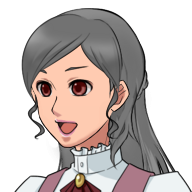
\includegraphics[width=\textwidth]{\jumpakuasset/A.png}\caption{恵伊}\label{fig:jumpakuA}\end{minipage}
\begin{minipage}{0.2\textwidth}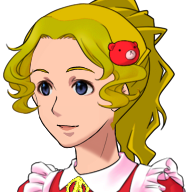
\includegraphics[width=\textwidth]{\jumpakuasset/B.png}\caption{美衣}\label{fig:jumpakuB}\end{minipage}
\begin{minipage}{0.2\textwidth}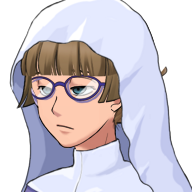
\includegraphics[width=\textwidth]{\jumpakuasset/C.png}\caption{史衣}\label{fig:jumpakuC}\end{minipage}
\begin{minipage}{0.2\textwidth}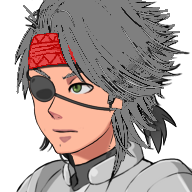
\includegraphics[width=\textwidth]{\jumpakuasset/D.png}\caption{出井}\label{fig:jumpakuD}\end{minipage}\\
\begin{minipage}{0.2\textwidth}
\includegraphics[width=\textwidth]{\jumpakuasset/E.png}\caption{良威}\label{fig:jumpakuE}\end{minipage}
\begin{minipage}{0.2\textwidth}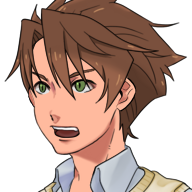
\includegraphics[width=\textwidth]{\jumpakuasset/F.png}\caption{恵夫}\label{fig:jumpakuF}\end{minipage}
\begin{minipage}{0.2\textwidth}
\includegraphics[width=\textwidth]{\jumpakuasset/G.png}\caption{寺井}\label{fig:jumpakuG}\end{minipage}
\begin{minipage}{0.2\textwidth}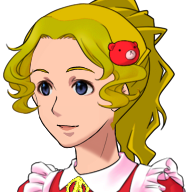
\includegraphics[width=\textwidth]{\jumpakuasset/B.png}\caption{永一}\label{fig:jumpakuH}\end{minipage}\\
\begin{minipage}{0.2\textwidth}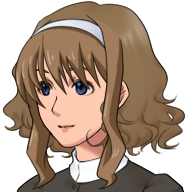
\includegraphics[width=\textwidth]{\jumpakuasset/Me.png}\caption{愛}\label{fig:jumpakuI}\end{minipage}
\begin{minipage}{0.2\textwidth}
\includegraphics[width=\textwidth]{\jumpakuasset/JumpakuMark_250x250.png}\caption{Jumpaku}\label{fig:jumpakuJ}\end{minipage}
\end{tabular}
\end{figure}
彼らの詳しい過去についてはここでは省略するが
\footnote{\href{http://jumpaku.hatenablog.com/entry/2016/04/14/002437}{\underline{愛と血の\ruby[g]{修羅場}{サスペンス}}},
\href{http://jumpaku.hatenablog.com/entry/2016/07/24/032632}{\underline{恋と友情の\ruby[g]{常識}{ファイト}}}および
\href{http://jumpaku.hatenablog.com/entry/2017/07/24/044918}{\underline{罪と幸せの\ruby[g]{四苦八苦}{ノアズアーク}}}をプレイしてください.},
既にこのうち5人が死んでいる.
まず,寺井が恵夫に殺された.
次に,良威が恵伊に殺され,私は報復した.
さらに,恵夫が史衣に殺され,私はまた報復した.
残ったのは,私,美衣,出井,永一の4人だけだった.

美衣,出井,永一の関係を簡単に紹介しておく.
美衣と永一は2人の人格で1つの体を共有しているが,私は2人として扱っている.
また,美衣と永一は姉弟である.
そして,出井と美衣はこの前結婚した.
彼らは生きる希望に満ち溢れていた.

\section{愛の事件}
それはまさに不可能犯罪だった.
密室にいた美衣,出井,永一の3人が消された.
跡形もなく消滅していた.
どのようにそれがなされたのかは分からないし,解明されることも無いだろう.
現場に残されたのはは血文字で書かれた不完全なダイイングメッセージだけだった.

「犯人は...」

\section{愛の決意}
事実は小説より奇なり.
密室より人間が消失した.
現実の世界でそんなことが発生するのだろうか?
いや,しない.
私が現実だと思って生きてきたこの世界は,夢,ゲームまたは小説の中の世界なのかもしれない.
それは,人間が密室から消えるという事象は現実に発生するとは考えられないからだ.
現実の世界で発生しえない事象が発生したなら,その世界は現実の世界ではない.
逆に,この世界が現実ではないとすると,現実で発生しえない事象でも発生しうる.
世界の枠組みを考え直せば,不可能なものが可能となることがあるのだ.
例えば,現実の世界という枠組みの中では人が消える事は無いが,もし小説の世界という枠組みなら人が消えることもある.
私がこれまで現実と思ってきた世界は,実は小説の世界なのかもしれない.
これを現実と確かめる事はできない.
まさに胡蝶の夢である.

しかし,真実を追い求める探偵は,世界の枠組みを考え直すだけで変わってしまうような些細なことに惑わされてはいけない.
探偵が真実を求める際に武器にできるのは論理的な推論しか無いのだ.
前提条件から論理的に推論された結論は,例えこの世界がどのような世界であっても揺らがない.
そのような結論が,探偵が追い求めるべき真実なのだ.
例え,犯人が未登場の者,中国人,探偵自身,双子,複数犯,捜査員,端役,プロの犯罪者または被害者自身であったとしても,
例え,犯行が秘密の通路もしくは隠し部屋,未発見の毒薬,難解な説明を要し,もしくは未来に登場する科学技術または超自然の術によって行われたとしても,
例え,動機が不明瞭であったり,状況に説得力が無かったとしても,
探偵は論理的な推論によって結論を導き,これを真相としなくてはいけない.

\section{愛の推理}
誰かが3人を消したのか?
それとも,3人の中の誰かが犯人で,被害者を消した後,隠れ続けているのか?
まず,私は犯行機会のあった容疑者として私自身,美衣,出井,永一の4人を挙げた.

その上で,美衣と永一が2心同体であったこと,
出井と美衣が愛し合っていたこと,
自分の行動の記憶,
その他3人の性格等を考慮した結果,以下の主張が成り立つと結論付けた.
\begin{itemize}
\item 私は犯人ではなく被害者でもない.
\item 美衣が犯人ならば永一も犯人である.
\item 美衣が被害者ならば永一も被害者である.
\item 容疑者のうち犯人であり被害者でもある者はいない.
\item 容疑者のうち犯人または被害者である者は3人である.
\item 出井は犯人ではない.
\item 美衣が犯人ならば出井は被害者ではない.
\end{itemize}

これらの主張に基づいて,私は上の容疑者のうち犯人は誰なのか,容疑者のうち被害者は誰なのか,
といった真相を論理的に導いた\footnote{ヒントとして,真実を導くプログラムの例を\ref{section:jumpakuprogram}に示す.}.
\begin{description}
\item[容疑者のうち犯人は愛であり, 被害者は出井である.] \ref{section:jumpakufailure1}へ進む.
\item[容疑者のうち犯人は愛であり, 被害者は出井,愛である.] \ref{section:jumpakufailure2}へ進む.
\item[容疑者のうち犯人は愛であり, 被害者は美衣,出井,永一である.] \ref{section:jumpakufailure3}へ進む.
\item[容疑者のうち犯人は永一であり, 被害者は愛である.] \ref{section:jumpakufailure4}へ進む.
\item[容疑者のうち犯人は永一であり, 被害者は美衣,愛である.] \ref{section:jumpakufailure5}へ進む.
\item[容疑者のうち犯人は永一,愛であり, 被害者は美衣,出井,愛である.] \ref{section:jumpakufailure6}へ進む.
\item[容疑者のうち犯人は出井であり, 被害者は愛である.] \ref{section:jumpakufailure7}へ進む.
\item[容疑者のうち犯人は出井であり, 被害者は出井,永一,愛である.] \ref{section:jumpakufailure8}へ進む.
\item[容疑者のうち犯人は出井,愛であり, 被害者は愛である.] \ref{section:jumpakufailure9}へ進む.
\item[容疑者のうち犯人は出井,永一であり, 被害者は美衣である.] \ref{section:jumpakufailure10}へ進む.
\item[容疑者のうち犯人は出井,永一,愛であり, 被害者は出井,永一,愛である.] \ref{section:jumpakufailure11}へ進む.
\item[容疑者のうち犯人は美衣,永一であり, 被害者は美衣,永一である.] \ref{section:jumpakufailure12}へ進む.
\item[容疑者のうち犯人は美衣,永一であり, 被害者は美衣,出井である.] \ref{section:jumpakufailure13}へ進む.
\item[容疑者のうち犯人は美衣,永一,愛であり, 被害者は美衣,愛である.] \ref{section:jumpakufailure14}へ進む.
\item[容疑者のうち犯人は美衣,永一,愛であり, 被害者は美衣,出井である.] \ref{section:jumpakufailure15}へ進む.
\item[容疑者のうち犯人は美衣,出井であり, 被害者は出井である.] \ref{section:jumpakufailure16}へ進む.
\item[容疑者のうち犯人は美衣,出井であり, 被害者は出井,永一である.] \ref{section:jumpakufailure17}へ進む.
\item[容疑者のうち犯人は美衣,出井,愛であり, 被害者は愛である.] \ref{section:jumpakufailure18}へ進む.
\item[容疑者のうち犯人は美衣,出井,愛であり, 被害者は美衣,出井,愛である.] \ref{section:jumpakufailure19}へ進む.
\item[容疑者のうち犯人は美衣,出井,永一であり, 被害者は美衣,出井である.] \ref{section:jumpakufailure20}へ進む.
\item[容疑者のうち犯人は美衣,出井であり, 被害者はいない.] \ref{section:jumpakufailure21}へ進む.
\item[容疑者の中に犯人はおらず,容疑者のうち被害者は美衣,出井,永一である.] \ref{section:jumpakusuccess23}へ進む.
\item[容疑者の中に犯人は美衣,出井,永一であり,容疑者のうち被害者はいない.] \ref{section:jumpakufailure24}へ進む.
\item[容疑者の中に犯人はおらず,容疑者のうち被害者もいない.] \ref{section:jumpakufailure25}へ進む.
\item[容疑者のうち犯人はおらず, 被害者は永一である.] \ref{section:jumpakufailure26}へ進む.
\item[容疑者のうち犯人はおらず, 被害者は出井,永一である.] \ref{section:jumpakufailure27}へ進む.
\end{description}
\newpage

\subsection{失敗}\label{section:jumpakufailure1}間違えた.探偵失敗だ.失敗END...\ref{section:jumpakubegin}へ戻る.\newpage
\subsection{失敗}\label{section:jumpakufailure2}間違えた.探偵失敗だ.失敗END...\ref{section:jumpakubegin}へ戻る.\newpage
\subsection{失敗}\label{section:jumpakufailure3}間違えた.探偵失敗だ.失敗END...\ref{section:jumpakubegin}へ戻る.\newpage
\subsection{失敗}\label{section:jumpakufailure4}間違えた.探偵失敗だ.失敗END...\ref{section:jumpakubegin}へ戻る.\newpage
\subsection{失敗}\label{section:jumpakufailure5}間違えた.探偵失敗だ.失敗END...\ref{section:jumpakubegin}へ戻る.\newpage
\subsection{失敗}\label{section:jumpakufailure6}間違えた.探偵失敗だ.失敗END...\ref{section:jumpakubegin}へ戻る.\newpage
\subsection{失敗}\label{section:jumpakufailure7}間違えた.探偵失敗だ.失敗END...\ref{section:jumpakubegin}へ戻る.\newpage
\subsection{失敗}\label{section:jumpakufailure8}間違えた.探偵失敗だ.失敗END...\ref{section:jumpakubegin}へ戻る.\newpage
\subsection{失敗}\label{section:jumpakufailure9}間違えた.探偵失敗だ.失敗END...\ref{section:jumpakubegin}へ戻る.\newpage
\subsection{失敗}\label{section:jumpakufailure10}間違えた.探偵失敗だ.失敗END...\ref{section:jumpakubegin}へ戻る.\newpage
\subsection{失敗}\label{section:jumpakufailure11}間違えた.探偵失敗だ.失敗END...\ref{section:jumpakubegin}へ戻る.\newpage
\subsection{失敗}\label{section:jumpakufailure12}間違えた.探偵失敗だ.失敗END...\ref{section:jumpakubegin}へ戻る.\newpage
\subsection{失敗}\label{section:jumpakufailure13}間違えた.探偵失敗だ.失敗END...\ref{section:jumpakubegin}へ戻る.\newpage
\subsection{失敗}\label{section:jumpakufailure14}間違えた.探偵失敗だ.失敗END...\ref{section:jumpakubegin}へ戻る.\newpage
\subsection{失敗}\label{section:jumpakufailure15}間違えた.探偵失敗だ.失敗END...\ref{section:jumpakubegin}へ戻る.\newpage
\subsection{失敗}\label{section:jumpakufailure16}間違えた.探偵失敗だ.失敗END...\ref{section:jumpakubegin}へ戻る.\newpage
\subsection{失敗}\label{section:jumpakufailure17}間違えた.探偵失敗だ.失敗END...\ref{section:jumpakubegin}へ戻る.\newpage
\subsection{失敗}\label{section:jumpakufailure18}間違えた.探偵失敗だ.失敗END...\ref{section:jumpakubegin}へ戻る.\newpage
\subsection{失敗}\label{section:jumpakufailure19}間違えた.探偵失敗だ.失敗END...\ref{section:jumpakubegin}へ戻る.\newpage
\subsection{失敗}\label{section:jumpakufailure20}間違えた.探偵失敗だ.失敗END...\ref{section:jumpakubegin}へ戻る.\newpage
\subsection{失敗}\label{section:jumpakufailure21}間違えた.探偵失敗だ.失敗END...\ref{section:jumpakubegin}へ戻る.\newpage
\subsection{失敗}\label{section:jumpakufailure22}間違えた.探偵失敗だ.失敗END...\ref{section:jumpakubegin}へ戻る.\newpage
\subsection{成功}\label{section:jumpakusuccess23}真実へ到達した.\ref{section:jumpakuresult}へ進む.\newpage
\subsection{失敗}\label{section:jumpakufailure24}間違えた.探偵失敗だ.失敗END...\ref{section:jumpakubegin}へ戻る.\newpage
\subsection{失敗}\label{section:jumpakufailure25}間違えた.探偵失敗だ.失敗END...\ref{section:jumpakubegin}へ戻る.\newpage
\subsection{失敗}\label{section:jumpakufailure26}間違えた.探偵失敗だ.失敗END...\ref{section:jumpakubegin}へ戻る.\newpage
\subsection{失敗}\label{section:jumpakufailure27}間違えた.探偵失敗だ.失敗END...\ref{section:jumpakubegin}へ戻る.\newpage

\section{愛の真相}\label{section:jumpakuresult}
真犯人は容疑者の中にはいない.
美衣,出井,永一は全員被害者だ.
これは論理的に導かれるたった一つの真相である.
例え,どんな理由があろうとも,
論理的な推論によって導かれる結論なのだから,これは真実なのだ.

\section{愛の飛躍}
探偵としての仕事が終わった.
ところが,私の思考は続いた.
失った仲間を思うと思考せずにはいられなかった.
3人を消した犯人は容疑者の中にはいない.
では,それ以外の誰なのか?
その思考は論理的な推論を飛躍した.

そもそも,
\begin{description}
\item[この世界は現実ではない.] \ref{subsection:jumpakulast1success}へ進む.
\item[この世界は現実である.] \ref{subsection:jumpakulast1failure}へ進む.
\end{description}
\newpage

\subsection{成功}\label{subsection:jumpakulast1success}なぜなら,密室から人間が消失する事は現実の世界では発生しないのだから.
次に,現実ではないこの世界は
\begin{description}
\item[何者かの意思によって作り出されている気がする.] \ref{subsection:jumpakulast2success}へ進む.
\item[ランダムに生成されている気がする.] \ref{subsection:jumpakulast2failure}へ進む.
\end{description}
\newpage

\subsection{失敗}\label{subsection:jumpakulast1failure}\ref{section:jumpakubegin}へ戻る.\newpage

\subsection{成功}\label{subsection:jumpakulast2success}
なぜなら,私の周りで殺人事件が多すぎること,
私を含めた仲間の名前がアルファベット順に並ぶことなど,不自然なことが多いから.

この世界を作り,私の仲間を消した犯人の名前の頭文字は
\begin{description}
\item[A] \ref{subsection:jumpakulast3failureA}へ進む.
\item[B] \ref{subsection:jumpakulast3failureB}へ進む.
\item[C] \ref{subsection:jumpakulast3failureC}へ進む.
\item[D] \ref{subsection:jumpakulast3failureD}へ進む.
\item[E] \ref{subsection:jumpakulast3failureE}へ進む.
\item[F] \ref{subsection:jumpakulast3failureF}へ進む.
\item[G] \ref{subsection:jumpakulast3failureG}へ進む.
\item[H] \ref{subsection:jumpakulast3failureH}へ進む.
\item[I] \ref{subsection:jumpakulast3failureI}へ進む.
\item[J] \ref{subsection:jumpakulast3successJ}へ進む.
\item[K] \ref{subsection:jumpakulast3failureK}へ進む.
\item[L] \ref{subsection:jumpakulast3failureL}へ進む.
\item[M] \ref{subsection:jumpakulast3failureM}へ進む.
\item[N] \ref{subsection:jumpakulast3failureN}へ進む.
\item[O] \ref{subsection:jumpakulast3failureO}へ進む.
\item[P] \ref{subsection:jumpakulast3failureP}へ進む.
\item[Q] \ref{subsection:jumpakulast3failureQ}へ進む.
\item[R] \ref{subsection:jumpakulast3failureR}へ進む.
\item[S] \ref{subsection:jumpakulast3failureS}へ進む.
\item[T] \ref{subsection:jumpakulast3failureT}へ進む.
\item[U] \ref{subsection:jumpakulast3failureU}へ進む.
\item[V] \ref{subsection:jumpakulast3failureV}へ進む.
\item[W] \ref{subsection:jumpakulast3failureW}へ進む.
\item[X] \ref{subsection:jumpakulast3failureX}へ進む.
\item[Y] \ref{subsection:jumpakulast3failureY}へ進む.
\item[Z] \ref{subsection:jumpakulast3failureZ}へ進む.
\end{description}
\newpage

\subsection{失敗}\label{subsection:jumpakulast2failure}\ref{section:jumpakubegin}へ戻る.\newpage

\subsection{失敗}\label{subsection:jumpakulast3failureA}\ref{section:jumpakubegin}へ戻る.\newpage
\subsection{失敗}\label{subsection:jumpakulast3failureB}\ref{section:jumpakubegin}へ戻る.\newpage
\subsection{失敗}\label{subsection:jumpakulast3failureC}\ref{section:jumpakubegin}へ戻る.\newpage
\subsection{失敗}\label{subsection:jumpakulast3failureD}\ref{section:jumpakubegin}へ戻る.\newpage
\subsection{失敗}\label{subsection:jumpakulast3failureE}\ref{section:jumpakubegin}へ戻る.\newpage
\subsection{失敗}\label{subsection:jumpakulast3failureF}\ref{section:jumpakubegin}へ戻る.\newpage
\subsection{失敗}\label{subsection:jumpakulast3failureG}\ref{section:jumpakubegin}へ戻る.\newpage
\subsection{失敗}\label{subsection:jumpakulast3failureH}\ref{section:jumpakubegin}へ戻る.\newpage
\subsection{失敗}\label{subsection:jumpakulast3failureI}\ref{section:jumpakubegin}へ戻る.\newpage
\subsection{成功}\label{subsection:jumpakulast3successJ}\ref{section:jumpakuending}へ進む.\newpage
\subsection{失敗}\label{subsection:jumpakulast3failureK}\ref{section:jumpakubegin}へ戻る.\newpage
\subsection{失敗}\label{subsection:jumpakulast3failureL}\ref{section:jumpakubegin}へ戻る.\newpage
\subsection{失敗}\label{subsection:jumpakulast3failureM}\ref{section:jumpakubegin}へ戻る.\newpage
\subsection{失敗}\label{subsection:jumpakulast3failureN}\ref{section:jumpakubegin}へ戻る.\newpage
\subsection{失敗}\label{subsection:jumpakulast3failureO}\ref{section:jumpakubegin}へ戻る.\newpage
\subsection{失敗}\label{subsection:jumpakulast3failureP}\ref{section:jumpakubegin}へ戻る.\newpage
\subsection{失敗}\label{subsection:jumpakulast3failureQ}\ref{section:jumpakubegin}へ戻る.\newpage
\subsection{失敗}\label{subsection:jumpakulast3failureR}\ref{section:jumpakubegin}へ戻る.\newpage
\subsection{失敗}\label{subsection:jumpakulast3failureS}\ref{section:jumpakubegin}へ戻る.\newpage
\subsection{失敗}\label{subsection:jumpakulast3failureT}\ref{section:jumpakubegin}へ戻る.\newpage
\subsection{失敗}\label{subsection:jumpakulast3failureU}\ref{section:jumpakubegin}へ戻る.\newpage
\subsection{失敗}\label{subsection:jumpakulast3failureV}\ref{section:jumpakubegin}へ戻る.\newpage
\subsection{失敗}\label{subsection:jumpakulast3failureW}\ref{section:jumpakubegin}へ戻る.\newpage
\subsection{失敗}\label{subsection:jumpakulast3failureX}\ref{section:jumpakubegin}へ戻る.\newpage
\subsection{失敗}\label{subsection:jumpakulast3failureY}\ref{section:jumpakubegin}へ戻る.\newpage
\subsection{失敗}\label{subsection:jumpakulast3failureZ}\ref{section:jumpakubegin}へ戻る.\newpage

\section{愛の終点}\label{section:jumpakuending}
私の世界を作り,私を生かし,仲間を奪ったのはこの物語を書いたJumpakuである.
動機はきっと「面白いと思ったから」だろう.
私は世界の理を理解した.

そして.

それでも.

もっと,生きよう.

解決END.
\newpage

\section*{サンプルコード}\label{section:jumpakuprogram}
以下に今回の事件の論理的推論を行うためのPython3のプログラムを示す.
\inputminted[linenos]{python3}{\jumpakuasset/LogicQuiz.py}
\end{comment}

\section*{あとがき}
本章にはBSD 2-Clause Licenseが適用されます.

\begin{quote}
BSD 2-Clause License

Copyright (c) 2018, Jumpaku
All rights reserved.

Redistribution and use in source and binary forms, with or without
modification, are permitted provided that the following conditions are met:
\begin{itemize}
\item Redistributions of source code must retain the above copyright notice, this
  list of conditions and the following disclaimer.
\item Redistributions in binary form must reproduce the above copyright notice,
  this list of conditions and the following disclaimer in the documentation
  and/or other materials provided with the distribution.
\end{itemize}
THIS SOFTWARE IS PROVIDED BY THE COPYRIGHT HOLDERS AND CONTRIBUTORS "AS IS"
AND ANY EXPRESS OR IMPLIED WARRANTIES, INCLUDING, BUT NOT LIMITED TO, THE
IMPLIED WARRANTIES OF MERCHANTABILITY AND FITNESS FOR A PARTICULAR PURPOSE ARE
DISCLAIMED. IN NO EVENT SHALL THE COPYRIGHT HOLDER OR CONTRIBUTORS BE LIABLE
FOR ANY DIRECT, INDIRECT, INCIDENTAL, SPECIAL, EXEMPLARY, OR CONSEQUENTIAL
DAMAGES (INCLUDING, BUT NOT LIMITED TO, PROCUREMENT OF SUBSTITUTE GOODS OR
SERVICES; LOSS OF USE, DATA, OR PROFITS; OR BUSINESS INTERRUPTION) HOWEVER
CAUSED AND ON ANY THEORY OF LIABILITY, WHETHER IN CONTRACT, STRICT LIABILITY,
OR TORT (INCLUDING NEGLIGENCE OR OTHERWISE) ARISING IN ANY WAY OUT OF THE USE
OF THIS SOFTWARE, EVEN IF ADVISED OF THE POSSIBILITY OF SUCH DAMAGE.
\end{quote}

また,キャラクタの画像は罪と幸せの\ruby[g]{四苦八苦}{ノアズアーク}より引用しました.


\chapterauthor{あるねこ}
\chapter{関数型Python入門}
\section{はじめに}
どうも、みなさんおなじみのあるねこさんです。この記事ではPythonの型アノテーション機能を
活用し、型の力を借りつつPython上でHaskellライクな型クラスモデルを再現する方法を紹介します。また実際にPythonの型アノテーション機能を使う上でのメリットや注意点をその都度解説します。なお今回作成したものは僕のGithubリポジトリ\footnote{\url{https://github.com/aruneko/FunctionalPy}}に掲載してありますので、ぜひご利用ください。

それでは型の世界へレッツゴー!

\section{型とPythonとmypyと}
\subsection{Pythonにおける型ヒンティング}
あまりなじみがないかもしれませんが、Python3系では関数やその引数に型アノテーションを書くことができ、その機能はバージョンアップごとに強化されています。特にPython3.5ではtypingモジュールが追加されてジェネリックな型アノテーションを書けるようになり、3.6では個別の変数にも書くことができるようになりました。また、高階関数などもサポートされていて、多彩な型を表現できるようになっています。

ただしこれらの型アノテーションは実行時には完全に無視され、いかなる値が渡ってきてもチェックは行われません。あくまで人間や静的コード解析ツールにとってわかりやすくなるためだけの機能となっています。そのため、List[int]型に特化した以下のコードはList[str]を与えても何のエラーや警告も出さずに実行できます。

\inputpython{./assets/aruneko/sample01.py}

\subsection{mypyによる型の解析}
型チェックはmypyというツールを使って行います。あるいは、Pycharmにデフォルトで搭載されている型チェック機能も利用できます。ただしこれらのツールで同じコードを解析した際に同じ結果になるかは未検証です。この記事では特に断りが無い場合mypyを利用します。

mypyをインストールするにはpipコマンドを利用します。一昔前は``mypy-lang''パッケージとして登録されていましたが、現在は``mypy''パッケージに名称を変更しているので、過去の資料を参照する際は注意が必要です。

\begin{bashcode}
pip install mypy
\end{bashcode}

それではmypyでの解析を試してみましょう。まず先ほどのサンプルコードを解析します。mypyコマンドで解析したいファイル名を引数に指定することで解析することができます。今回は型エラーを発生させるコードを書いているため、型チェックの結果int型とstr型は合致しないというエラーが発生しています。

\begin{bashcode}
mypy sample01.py
sample01.py:9: error: List item 0 has incompatible type "str"; expected "int"
sample01.py:9: error: List item 1 has incompatible type "str"; expected "int"
sample01.py:9: error: List item 2 has incompatible type "str"; expected "int"
\end{bashcode}

それではジェネリックを使って先ほどのコードを書き直し、もう一度チェックを書けてみましょう。今回は型エラーが発生しないため、特に何も表示されずmypyが終了します。

\inputpython{./assets/aruneko/sample02.py}

\begin{bashcode}
mypy sample02.py
\end{bashcode}

このmypyによる型チェックをCIと組み合わせて、型を合致しないコードがコミットされたときにテストを通らないようにすることで想定外の関数の利用を制限し、より安全なコードを書くヒントを得ることができるメリットがあります。

これで基本的なmypyの使い方と型の書き方が説明できました。それではいよいよ型クラスを作っていきましょう。

\section{型クラスを作る}
\subsection{型クラス概要}
型クラスとは、その型クラスを実装した具象型がどう振る舞うべきかを定義したものです。JavaでいうInterfaceを想像するとわかりやすいかもしれません。

今回は特に有名な``Functor''、``Applicative''、``Monad''の3つの型クラスを実装します。これらの型クラスは継承関係にあり、ListやMaybe(ScalaのOption)などよく使われる型を抽象化することができます。それぞれの型クラスの詳細は実装時に詳しく説明します。

\subsection{Functor型クラスの実装}
Functorはリストなどの全要素に1引数関数を適用するmap関数をメソッドとして持っている型クラスです。まずFunctorのコードを紹介します。

\inputpython{./assets/aruneko/Functor.py}

先ほども述べたとおり、型クラスはいわゆるインターフェースと類似するものですので、PythonのABCパッケージを使って抽象クラスとして定義していきます。また、Functorはコンテナ的な性質を持つため、Generic[A]を継承してこれ自身がジェネリックな型であることを明示します。

続いて、mapメソッドの定義を記述します。mapメソッドは1引数関数を取ってそれを適用したFunctorを返すため、Callableを用いて型宣言を行います。ただしPythonではクラスの定義中に自分自身のクラス名を利用することができないため、mypyやPyCharmがサポートしているコメントによる型記法を利用します。またmapは抽象メソッドで実装を持たないため、passを書いて実装がないことを明示します。

\subsection{Applicative型クラスの実装}
続いてApplicative型クラスを定義しましょう。この型クラスは本来``pure''と``ap''の2つのメソッドを持つべきです。しかし``pure''はある値をアプリカティブ値にするための関数で、これは各クラスが``\verb+__init__+''メソッドを実装するだけで実現できてしまいます。従って今回は手抜きをして``ap''だけをApplicativeのメソッドとして定義します。

では``ap''メソッドが何者かと言いますと、1引数関数が入ったApplicative値を引数にとって、その関数にApplicative値の中身に入っている値を適用する関数です。言葉で説明するのも難しいので、さっそく型定義を見てみましょう。

\inputpython{./assets/aruneko/Applicative.py}

まず大前提としてApplicativeはFunctorとして振る舞うこともできるためFunctorを継承するところから始めます。そしてネストが深い上に長くて読みづらいですが、1引数関数を値として持つApplicative値を引数にとってApplicative値を返すという型を書いておきます。

\subsection{Monad型クラスの実装}
最後にMonad型クラスを定義しましょう。Monadと聞くと身構える人もいるかもしれませんが、きちんと説明しますので大丈夫です。さっそく実装を見てみましょう。

\inputpython{./assets/aruneko/Monad.py}

Monad型クラスはいわゆる``\verb+flat_map+''をメソッドに持つ型クラスです。``\verb+flat_map+''はMonad値を返す1引数関数を引数にとってMonad値に適用し、その際2重になったMonad値を剥がすメソッドです。本来であればApplicativeの``pure''と同じ働きをする関数もメソッドに持つべきですが、上記の理由により省略します。Monad型クラスもまたFunctorとして振る舞い、さらにApplicativeとしても振る舞うため、Applicative型クラスを継承しています。

ひとまずこれで今回ご紹介する型クラスの定義は終わったので、次はいよいよこれらの型クラスを具象クラスに実装していきます。

\section{List Monadを作る}
\subsection{ベースを作る}
それではさっそくList Monadのベースを作っていきます。既存のlistを継承し、Monad型クラスを実装します。ただし今回はtypingパッケージのListクラスと名前を被らせないために、Scalaに倣って``Seq''クラスと命名します。ひとまず機械的に作ってしまいましょう。以下のような実装になります。

\inputpython{./assets/aruneko/Seq01.py}

実装するメソッドの型宣言は今実装しているクラスに合わせて``Seq''に変更しておきます。また、``\verb+__init__+''の実装は可変長引数を受け取ってリストに詰め直す動作をするように作ってあります。こうすることでSeq専用のリテラルが追加されたかのように記述できます。

\subsection{各種型クラスの実装}
ではまずSeqをFunctorにするために、mapの実装をしていきます。といってもリスト内包表記を使えば良いのでとても簡単です。ここでのselfは自分が保持しているlistになっているため、selfを直接イテレートさせればOKです。あとは引数にとってきた関数を適用して新たなリストを作成し、それを展開してもう一度Seqに詰め直せば完成です。

\inputpython{./assets/aruneko/Seq_map.py}

続いてSeqにApplicativeを実装するために、apの実装を考えます。apは引数に``1引数関数''のSeqを取ります。これをSeqに適用するわけですから、全要素数は``$\mbox{引数のリストの長さ} \times \mbox{対象のリストの長さ}$''になります。単純にループを回すだけでは実装できないので、少々気持ち悪いですが2重に回します。このように2重ループを回すことでSeqから取り出した関数に対してselfの値を取り出して適用していき、入れ子になっていないSeqを作り出します。

\inputpython{./assets/aruneko/Seq_ap.py}

では最後にflat\_mapを実装しましょう。これでSeqはMonadになることができます。今度も引数に取った関数がSeqを返してしまう都合上単純にループを回すと入れ子構造になってしまうため、それを防止するために2重ループを回します。selfから取り出した値を引数に取った関数に適用し、その結果を1つずつ取り出してリストにします。あとはSeqに詰め直して完成です。

\inputpython{./assets/aruneko/Seq_flat_map.py}

これでFunctor、Applicative、Monadに必要な全てのメソッドを実装できました。この時点でmypyを使って型検査を行いエラーがないことを確かめたいのですが、実はmypyにはインターフェースを実装したときの型検査にバグがあり、正しく実装をしているにもかかわらず親クラスと型が合わないという型エラーを出してしまいます。この問題についてはGithub上で議論されていますが\footnote{\url{https://github.com/python/typing/issues/241}}、今のところ解決していません。あまり気にしないでおきましょう。

\section{まとめ}
ここまでPython上で型を定義しながらMonad則を満たすSeqクラスを作ってきました。皆さんにはPythonで型を書き、それをチェックする方法を少しでも伝えられれば嬉しいです。また、その型の力を使ってMonadまで作れてしまうこともぜひ知っていただけるとありがたいです。

読者の皆さんもぜひ新規Pythonコードには型定義をしっかりと書いて、CIにmypyを組み込んでチェックしてみてください。数日後の自分がそのコードを読み返したときに型というヒントを得ることができ、きっと開発の手助けになると思います。それでは良き型ライフを!

\newpage
\myimpression[%
name=LOCAL Students\\情報ボーイズの寄稿ノート, %
author=うっひょい, \and %
ちくうぇいと, \and %
あわあわ, \\ \and %
けんつ, \and %
さわだ, \and %
Jumpaku, \and %
あるねこ, %
date=2018年4月22日, %
publisher=LOCAL学生部, %
print=有限会社ねこのしっぽ %
]%
\end{document}
